\documentclass{ruthesis}
\special{papersize=8.5in,11in} % for A4-default configurations on servers


\usepackage[utf8]{inputenc}
\usepackage{longtable}
\usepackage{graphicx}
\usepackage{amssymb,amsmath,amsfonts}
\usepackage{amsbsy}
\usepackage[utf8]{inputenc}
\usepackage{array}
\usepackage{booktabs}
\usepackage{algorithm2e}
\usepackage{listings}
\usepackage{cleveref}
\usepackage{acronym}
\usepackage{subcaption}

\acrodef{QoS}{Quality of Service}
\acrodef{VM}{Virtual Machine}
\acrodef{UDF}{User Defined Function}
\acrodef{DAG}{Directed Acyclic Graph}
\acrodef{CEP}{Complex Event Processing}
\acrodef{IoT}{Internet of Things}
\acrodef{DSPE}{Data Stream Processing Engine}
\acrodef{DSP}{Data Stream Processing}
\acrodef{FCFS}{First-Come, First-Served}
\acrodef{SPDG}{Series-Parallel-Decomposable Graphs}
\acrodef{IPS}{Instructions per Second}
\acrodef{RTR}{Response Time Rate}
\acrodef{CR+RP}{Cost Rate with Region Patterns}
\acrodef{CI}{Cloud Infrastructure}
\acrodef{EI}{Edge Infrastructure}
\acrodef{LB}{Taneja et. al.}
\acrodef{DSP}{Distributed Stream Processing}
\acrodef{MIPS}{Millions of Instructions per Second}
\acrodef{SDN}{Software Defined Network}
\acrodef{SoC}{System on a Chip}
\acrodef{CDF}{Cumulative distribution function}
\acrodef{OODA}{Observe Orient Decide Act}

% set the default code style
\lstset{
    frame=tb, % draw a frame at the top and bottom of the code block
    tabsize=1, % tab space width
    showstringspaces=false, % don't mark spaces in strings
    basicstyle=\small,
    keywordstyle=[1]\color{green},
    keywordstyle=[2]\color{orange},
    keywordstyle=[3]\color{blue},
}

\lstdefinelanguage{mylang}{
  alsoletter={*,", 10, >=, :, 74,40,-},
  keywords=[1]{placement, minEndToEndLatency, minDataTransferRate, minMessagingCost},
  keywords=[2]{core, edge, *},
  keywords=[3]{new},
}

\begin{document}
\phd

%\title{Enabling Data-driven Stream Processing Pipelines for Edge Computing}
\title{Programming and Managing stream processing applications between the edge and the cloud}
\author{Eduard Gibert Renart}
\program{Computer Science}
\director{Manish Parashar}
\approvals{4}
\submissionyear{2017}
\submissionmonth{May}

\abstract{Due to the proliferation of the Internet of Things (IoT), the number of devices connected to the Internet is growing. These devices are generating unprecedented amounts of data at the edge of the infrastructure. Although the generated data provides great potential, identifying and processing relevant data points hidden in streams of unimportant data, and doing this in near real time, remains a significant challenge. Existing stream processing platforms require the data to be transported to the cloud for processing, resulting in latencies that can prevent timely decision making or may reduce the amount of data processed.


To address these challenges, this dissertation presents an IoT Edge Framework, called R-Pulsar, that extends cloud capabilities to local devices and provides a programming model for deciding what, when, where and how data get collected and processed. This thesis makes the following contributions: (1) A content- and location-based programming abstraction for specifying \textbf{what} data gets collected and \textbf{where} the data gets analyzed. (2) A rule-based programming abstraction for specifying \textbf{when} to trigger data-processing tasks based on data observations. (3) A programming abstraction for specifying \textbf{how} to split a given dataflow and place operators across edge and cloud resources. (4) An operator placement strategy that aims to minimize an aggregate cost which covers the end-to-end latency (time for an event to traverse the entire dataflow), the data transfer rate (amount of data transferred between the edge and the cloud) and the messaging cost (number of messages transferred between edge and the cloud). (5) Performance optimizations on the data-processing pipeline in order to achieve real-time performance on constrained devices.

The applicability of this work to real-world IoT applications is validated through a series of experiments where 

heterogeneous, geographically distributed services are composed based on user, resource provider, and application specifications. The results establish the potential impact of a system capable of real-time adaptability to changes in mixed resource environments, including multiple clouds, grids, clusters, supercomputers, and traditional data centers.



(6) An implementation of the above capabilities as part of the R-Pulsar software stack and its evaluation using embedded devices (Raspberry Pi and Android phone)}

\beforepreface
\acknowledgements{The body of the acknowledgements}
\dedication{The body of the dedication}
\afterpreface

\listoftables
\listoffigures

\chapter{Introduction}
\section{Challenges of IoT Applications}
IoT data features several all the Vs of BigData:
\begin{itemize}
    \item Volume: 
    \item Velocity:
    \item Variety: 
    \item Veracity: 
\end{itemize}

In addition IoT introduces a new set of challenges that big data does not have. The main challenges associated with the development and deployment of IoT analytics applications are:

\begin{itemize}
    \item Data heterogeneity:
    \item Real-time nature:
    \item Time and location dependencies:
    \item Privacy and security sensitivity:
\end{itemize}

%\section{IoT Application Lifecycle}
%The IoT application lifecycle comprises of the following phases: 

%\begin{itemize}
%    \item Data Collection:
%    \item Data Analysis:
%    \item Data Storage:
%\end{itemize}

\section{Motivation}

Due to the proliferation of the Internet of Things (IoT) paradigm, the number of devices connected to the Internet is growing. These devices are generating unprecedented amounts of data at the edges of the infrastructure. Although the generated data provides great potential, identifying and processing relevant data points hidden in streams of unimportant data, and doing this in near real time, remains a significant challenge. Existing stream processing platforms require the data to be transported to the cloud for processing, resulting in latencies that can prevent timely decision making or may reduce the amount of data processed.



\section{Problem Description}
\section{Overview of Thesis Research}
\section{Contributions}
This dissertation makes the following contributions:
\begin{itemize}
  \item A content- and location-based programming abstraction for specifying \textbf{what} data gets collected and \textbf{where} the data gets analyzed.
  \item A rule-based programming abstraction for specifying \textbf{when} to trigger data-processing tasks based on data observations.
  \item A programming abstraction for specifying \textbf{how} to split a given dataflow and place operators across edge and cloud resources.
  \item An operator placement strategy that aims to minimize an aggregate cost which covers the end-to-end latency (time for an event to traverse the entire dataflow), the data transfer rate (amount of data transferred between the edge and the cloud) and the messaging cost (number of messages transferred between edge and the cloud).
  \item Performance optimizations on the data-processing pipeline in order to achieve real-time performance on constrained devices.
  \item An implementation of the above capabilities as part of the R-Pulsar software stack and its evaluation using embedded devices (Raspberry Pi and Android phone).
\end{itemize}

\section{Outline}
The rest of this thesis is organized as follows.

Chapter 2 shows the benefits of using data staging, as well as motivating and representative workflow examples. This chapter also summarizes the key parameters and components of coupled scientific workflows.

Chapter 3 presents an overview of related research work.

Chapter x summarizes the research work of this thesis and presents future research
directions.
\chapter{Motivating Applications and Requirements}
\section{Emergence, Benefits and Limitations of Using Edge Computing}

\begin{table*}[t]
\caption{Edge Computing use cases, current limitations, and imperatives}
\label{tab:use_case}
\begin{tabular}{|c|c|c|c|}
\hline
Applications                  & Example Use Case                                                                                                                                                                     & Limitations                                                                                                                                                      & Requirements                                                                                                                                       \\ \hline
Smart City                & \begin{tabular}[c]{@{}c@{}}Help autistic people \\ navigate through large \\ crowded spaces.\end{tabular}                                                                        & \begin{tabular}[c]{@{}c@{}}Hard to provide real-time \\ directions due to the need to \\ send large volumes of data to \\ the cloud.\end{tabular}                & \begin{tabular}[c]{@{}c@{}}Low Latency, Security,\\ Geographically \\ Distributed,\\ Mobility, Scalability\\ Reliability and Robustness\end{tabular} \\ \hline
\begin{tabular}[c]{@{}c@{}}Disaster \\ Recovery\end{tabular}        & \begin{tabular}[c]{@{}c@{}}Need to quickly determine \\ whether  building conditions \\ are safe for  evacuees to return \\ after a natural  disaster \\ has struck.\end{tabular} & \begin{tabular}[c]{@{}c@{}}Hard to perform real-time \\ decision due to the need to \\ send large volumes of data to \\ the cloud.\end{tabular}                  & \begin{tabular}[c]{@{}c@{}}Low Latency,\\ Geographically  \\ Distributed,\\ Orchestration \\ and Management\end{tabular}                                 \\ \hline
\begin{tabular}[c]{@{}c@{}}Distributed \\ Observatories\end{tabular} & \begin{tabular}[c]{@{}c@{}}Large networked system of \\ under water instruments \\ to collect real-time data \\ from the ocean.\end{tabular}                                   & \begin{tabular}[c]{@{}c@{}}Hard to deliver near \\ real-time data to the end user \\ due to the need to send large\\  volumes of data to the cloud.\end{tabular} & \begin{tabular}[c]{@{}c@{}}Low Latency, Security,\\ Geographically \\ Distributed,\\ Multi-Tenancy, Scalability\end{tabular}                         \\ \hline
\begin{tabular}[c]{@{}c@{}}Video \\ Analaytics\end{tabular}          & \begin{tabular}[c]{@{}c@{}}Video analytics for safety \\ and security from public \\ video cameras.\end{tabular}                                                                & \begin{tabular}[c]{@{}c@{}}Hard to perform real-time \\ analytics due to the need to \\ send large volumes of data to \\ the cloud.\end{tabular}                 & \begin{tabular}[c]{@{}c@{}}Low Latency, Security,\\ Geographically \\ Distributed,\\ Scalability\end{tabular}                                        \\ \hline
\end{tabular}
\end{table*}


\section{Motivating Applications}\label{sec:usecases} 
IoT applications are present in several domains: Precision medicine, Urban mobility, and Healthcare.
In this section, we highlight four different use cases described in both industry and academia that benefits from the IoT paradigm. 
Table~\ref{tab:use_case} summarises the scenario, limitations and requirements of those use cases.

%To better understand the need for an edge middleware, this section presents four scenarios to motivate the need.

\subsection{Smart City}

The first use case is smart cities for people with disabilities. Large cities are difficult to navigate, especially for people with special needs such as those with visual impairment, Autism Spectrum Disorder (ASD), or simply those with navigational challenges. The primary objective of this application use case is to explore the use of IoT capabilities to transform cities around the world into smart cities capable of providing location-aware services (e.g., finding buildings and streets, improving travel experience, obtaining security alerts). In order to create smart cities that can support reliable navigation services to people with special needs, researchers are creating complex workflows integrating a number of novel IoT elements, including video analytics, Bluetooth beacons, mobile computing, and LiDAR-scanned 3D semantic models. For example, we may have a streaming application workflow that analyzes video feeds from the surveillance cameras of the streets in real-time to evaluate the density of crowds in different parts of the city to help select path choices. Especially, ASD individuals may prefer to choose paths that have less dense crowds due to psychological factors; people with visual impairment try to avoid large open spaces due to the difficulty of finding references for localization, and people in wheelchairs can navigate along paths with fewer crowds far more conveniently than among those with large crowds. This information is then combined with a 3D model and the location of the user to calculate the best path to reach the desired destination. Additionally, we need to continuously monitor the user (e.g., using the Bluetooth beacons), and the streets (e.g., using surveillance cameras) to adapt to changes. In the smart city use case, since there are multiple video cameras in different locations, sending the video feeds of this camera to the cloud will incur high latencies, bandwidth congestions, and privacy concerns.

\subsection{Disaster Recovery}

Our second use case is a disaster response use case. Disaster management is a process that involves four phases: mitigation, preparedness, response, and recovery. Mitigation efforts attempt to prevent hazards from developing into disasters altogether or to reduce the effects of disasters when they occur. In the preparedness phase, emergency managers develop plans of action when the disaster strikes and analyze and manage the required resources. The response phase executes the action plans, which include the mobilization of the necessary emergency services and dispatch of first responders and other material resources in the disaster area. Finally, the aim of the recovery phase is to restore the affected area to its previous state. This workflow focuses on the response phase by using a multi-stage generic response workflow that will be executed at the edge and at the core of the network. The workflow starts by capturing real-time data of the affected zones (e.g LiDAR, photogrammetry, etc.) and we perform a pre-processing stage at the edge of the network. In our case, a minivan or a drone with networking and computational capabilities will be used to determine the content of the data and if any further post-processing is needed. If further processing is needed, data will be either sent to the cloud to perform a change detection with previously recorded historical data, store data into the cloud, or notify agencies to determine if building conditions are safe. In the disaster recovery use case, the mapping of an affected area can have a total of 741 images and total 3.7 GB, with the biggest image 33.8 MB and the smallest 1.8 KB, taking over 1 hour to transfer all the data to the cloud with a 4G connection.

\begin{figure}[ht]
  \centering
  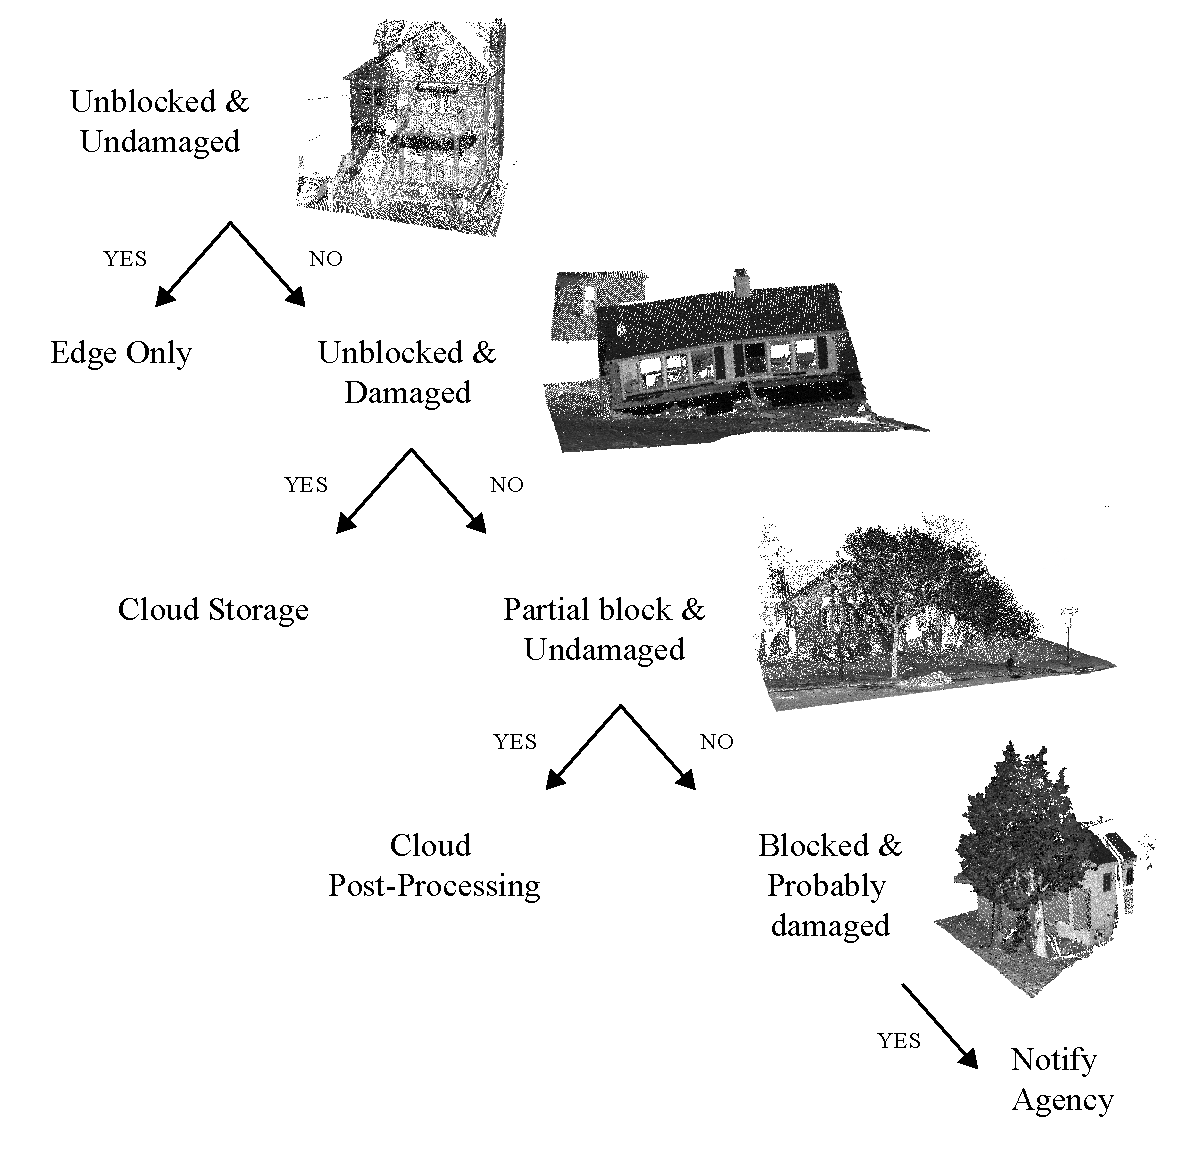
\includegraphics[width=0.5\linewidth]{Figures/diagonal.pdf}
  \caption{Disaster recovery decision stages and its associated reactions based on the LiDAR images.}
  \label{data_uncertainty}
\end{figure}

\subsection{Scientific Observatory}

It's a networked ocean research observatory with arrays of instrumented water column moorings and buoys, profilers, gliders, and autonomous underwater vehicles within the different open ocean and coastal regions. OOI infrastructure also includes a cabled array of instrumented seafloor platforms and water column moorings on the Juan de Fuca tectonic plate. This networked system of instruments, moored and mobile platforms, and arrays provide ocean scientists, educators, and the public the means to collect sustained, time-series data sets to enable the examination of complex, interlinked physical, chemical, biological, and geological processes operating throughout the coastal regions and open ocean. OOI implements a geographically distributed, secure, highly available CI that is responsible for data acquisition/collection, data storage and processing, and on-demand delivery of data and data products to scientists and application developers. The use of a well-defined API based on standard protocols enables other systems to interface and interact with OOI CI programmatically. The scientific observatory use case has a similar problem to the disaster recovery use case where the data is to big to send to the cloud in order to offer real-time data delivery.

\subsection{Video Analytics} 

The last use case is the use of video analytics~\cite{8358733} for safety and security. In video analytics, a single video camera can produce about 25-30 frames/second. In HD and FHD cameras an 8-bit uncompressed RGB frame amounts to about 553 Mbps and 1.24 Gbps for a one minute video, respectively. With the advent of 4k and 3D video cameras, this size is likely to grow exponentially. Developers and engineers are facing the challenge of providing on-time analytics of video data to support public safety and security from video cameras. Cloud computing is not efficient enough to support prompt analytics of such video data~\cite{7488250}. Video Analytics based on edge computing is the only feasible approach to cater to low latency requirement for large-scale video streams~\cite{8057318}.

\subsection{Observe Orient Decide Act Loop}

The \ac{OODA} loop refers to the decision-making cycle of observe, orient, decide, and act, developed by military strategists and the United States Air Force~\cite{OODA}. \ac{OODA} is a decision-making cycle to process data streaming from sensors in real time, becoming an essential design characteristic for IoT applications. 
\begin{figure}[h!]
  \centering
  \includegraphics[width=0.8\columnwidth]{Figures/ooda.pdf}
  \caption{RIoTBench IoT high-level logical interactions between different sensors, applications and users.}
  \label{fig:etl}
\end{figure}

Anshu \textit{et al.}~\cite{RIoTBench} offer a suite of IoT applications that follows the closed-loop \ac{OODA} cycle. The applications are based on common IoT patterns for data pre-processing, statistical summarization, and predictive analytics. These are coupled with workloads sourced from real IoT observations. A high-level overview of the logical interaction of the IoT applications is depicted in Figure~\ref{fig:etl}.

\textbf{Extract-Transform-Load (ETL)} consumes data from hundreds of thousands of edge sensors, and pre-processes, cleans, and archives the data. Further, the results are published to an edge broker so that clients interested in real-time monitoring can subscribe to it, while a copy is forked to the cloud for storage, and another to the next dataflow step.

\textbf{Statistical Summarization (STATS)} performs higher order aggregation and plotting operations, and stores the generated plots into the cloud, from where webpages can load the visualization files on browsers. 

\textbf{Model Training (TRAIN)} periodically loads the stored data from ETL step and trains forecasting models that are stored in the cloud, and notifies the message broker of an updated model being available. 

\textbf{The Predictive Analytics (PRED)} subscribe to the message broker and downloads the new models from the cloud, and continuously operates over the pre-processed data stream from ETL to make predictions and classifications that can indicate actions to be taken on the domain. It then notifies the message broker of the predictions, which can independently be subscribed to by a user or device for action. 

The ETL dataflow requires a low-latency cycle in order to achieve real-time monitoring, in addition it also requires some of its operators to be located in the cloud for storing messages and others to be at the edge of the network. This makes the ETL workflow the perfect candidate workflow for testing the operator placement strategy proposed. 
\chapter{Background and Related Work}
\section{Introduction}
Cloud computing was introduced a decade ago with the promise of seemingly infinite computing resources available on demand \cite{Armbrust09abovethe}. This model has proved to be effective for scaling up search engines\cite{7073834}, social networks\cite{6596496}, and content service providers\cite{6915771} to billions of users around the world. However, this centralized model is being challenged by the emergence of a new computing paradigm and associated technologies i.e. Internet of Things (IoT).

The Internet of Things paradigm (IoT) fosters the connection of large numbers of sensors to the network. According to Cisco systems~\cite{ciscoGlance}, 500 billion IoT devices are expected to be connected to the Internet by 2030, and mearly 50\% of the data produced worldwide will be generated by IoT sensors~\cite{McAuley}. As the volume of data generated from the devices increases, moving data from the edge of the network to the Cloud might not be feasible due to bandwidth constraints~\cite{8289317}. Furthermore, as low latency and location-aware applications emerge~\cite{7389122}, transfering all the data to the Cloud will not satisfy the low latency or location-aware constraints that the IoT applications expect. In addition, some applications, deal with sensitive and personal data, making it not possible to send the data to the Cloud due to privacy concerns~\cite{7849185}. For example, Toyota estimates that the amount of data flowing between vehicles and servers will reach 10 exabytes per month by 2025~\cite{Toyota}. Another example is commercial jets, which generate 10 TB of data for every 30 minutes of flight, making it impractical to transport all the data from the edge to the Cloud~\cite{ciscoJet}. 

Edge computing has emerged as a potential approach for handling the large quantity of data generated by connected devices. It leverages the ability to execute computations and process data at the edge of the network, closer from the location of data producers. Edge computing leverages smaller servers or single board computers that are widely distributed close to the edge to improve delays. Edge middleware is the essential software stack that serves as an interface between the Cloud and the IoT devices, supporting data discovery, communication and processing between edge devices and cloud services. %\hl{In this context, edge middleware platforms were created to ease the IoT application development by providing the necessary tools.} 

The realization of edge-based middleware platforms presents several conceptual and technical challenges. We believe that the seamless integration of edge and Cloud systems is one of the main challenges that prevent the efficient utilization of IoT. Without such an integration, developers must explicitly manage the platform as a unified set of resources to orchestrate computations, coordinate devices, and deliver data to users. As a result, there has been a substantial amount of research towards building edge-based middleware, addressing key crosscutting challenges, such as device discovery, scalability, and privacy and security. It is therefore important to understand the current state-of-the-art edge-based middleware and identify the gaps that may exist.

\begin{figure}[hbt!]
    \centering
    \includegraphics[scale=0.7]{Figures/IoTArchW.pdf}
    \caption{Edge-based middleware reference architecture consisting of four layers, each of them with their respective components.}
    \label{fig:EdgeArch}
\end{figure}

\section{Edge-based Middleware Architecture}\label{sec:arch}

Extensive research and development have been put into creating edge-based middleware systems. There are currently more than 100 edge-based middleware platforms in the market today and the number is continuously growing~\cite{List}. However, not every platform is designed with the same capabilities or architecture. Despite the diversity and large number of edge-based middleware systems, two common architectures emerge:

The majority of IoT platform's architecture follows the Cloud-centric approach. They are built on the premise that ingestion, management, and processing of IoT data can be done in the Cloud, without any edge computing capabilities. Some examples are: Particle Cloud~\cite{Particle}, Salesforce IoT Cloud~\cite{Salesforce_IoT_Cloud} and If This Then That~\cite{IFTTT}.

The other approach is the end-to-end architecture or edge-based middleware architecture built on the premise that edge-processing can save huge costs to clients. %An Internet of Things (IoT) gateway or middleware is a physical device that serves as the connection point between the Cloud and the edge sensors. The gateway or edge middlewares are, usually deployed on single board computers (e.g., Raspberry Pi's), minicomputers, or smart devices (e.g., smartphones, TVs, or refrigerators) to provide management, connectivity, and data pre-processing for sensors.

In this survey, we focus on the end-to-end or edge-based middleware architecture, since the Cloud-centric approach will not be able to satisfy the requirement of the IoT applications presented in section~\ref{sec:usecases}. In order to compare and contrast all the existing state-of-the-art edge-based middlewares, we carefully studied the requirements and limitations of the IoT applications and came up with a four-layer edge-based middleware framework that satisfies all the requirements and limitations of the IoT applications, and each of the middlewares should consist. Figure~\ref{fig:EdgeArch} presents the layers and components that need to be included in an edge-computing solution. The edge-based middleware architecture is composed of four separate layers: resource management, data processing, service , and security.

\begin{table}[hbt!]
\caption{Design goals of the resource management layer components of the cited papers in this survey.}
\label{tab:resource}
\resizebox{\textwidth}{!}{%
\begin{tabular}{c|c|c|c|c|c|c|}
\cline{2-7}
                                          & \multicolumn{2}{c|}{Resource Discovery}               & \multicolumn{2}{c|}{Resource Monitoring}              & \multicolumn{2}{c|}{Resource Mobility}                \\ \hline
\multicolumn{1}{|c|}{Paper}               & Distributed               & \begin{tabular}[c]{@{}c@{}}Low \\Overhead\end{tabular}             & Distributed               & \begin{tabular}[c]{@{}c@{}}Low \\ Overhead\end{tabular}              & Distributed               & \begin{tabular}[c]{@{}c@{}}Low \\ Overhead\end{tabular}              \\ \hline
\multicolumn{1}{|c|}{Paganelli et al.~\cite{article}}    & \checkmark & \checkmark &                           &                           &                           &                           \\ \hline
\multicolumn{1}{|c|}{Liu et al.~\cite{6680268}}          & \checkmark &                           &                           &                           &                           &                           \\ \hline
\multicolumn{1}{|c|}{Cirani et al.~\cite{6899579}}       & \checkmark & \checkmark &                           &                           &                           &                           \\ \hline
\multicolumn{1}{|c|}{Jara et al.~\cite{6550579}}         &                           & \checkmark &                           &                           &                           &                           \\ \hline
\multicolumn{1}{|c|}{Zhou et al.~\cite{6664533}}         &                           & \checkmark &                           &                           &                           &                           \\ \hline
\multicolumn{1}{|c|}{Tanganelli et al.~\cite{8086146}}   &                           &                           & \checkmark & \checkmark &                           &                           \\ \hline
\multicolumn{1}{|c|}{M{\"a}enp{\"a}{\"a} et al.~\cite{Maenpaa2012}}      &                           &                           & \checkmark & \checkmark &                           &                           \\ \hline
\multicolumn{1}{|c|}{SEGUE~\cite{SEGUE}}               &                           &                           &                           &                           & \checkmark & \checkmark \\ \hline
\multicolumn{1}{|c|}{Chaufournier et al.~\cite{Chaufournier:2017}} &                           &                           &                           &                           & \checkmark & \checkmark \\ \hline
\multicolumn{1}{|c|}{Farris et al.~\cite{Farris:2017}}        &                           &                           &                           &                           & \checkmark & \checkmark \\ \hline
\end{tabular}
}
\end{table}

\subsection{Resource Management Layer}
The resource management layer is dedicated to the discovery, identification and allocation of available resources. The challenge of the resource management layer is in managing these limited and geo-distributed resources efficiently. The resource management layer consists of the following components: resource discovery, resource monitoring, and resource mobility. Table~\ref{tab:resource} summarizes the design goals of each of the works focused on the resource management layer.

\subsubsection{Design Goals}

The following are the design goals that need to be taken into consideration when developing any of the components of the resource management layer.
\\\\
\textbf{Low Overhead:} The algorithms and protocols of the resource management layer need to offer low runtime overhead when deployed in performance-limited hardware platforms.
\\\\
\textbf{Distributed:} The resource management components also need to be designed in a distributed fashion in order to scale with the number of applications running in the system and with the number of IoT and edge devices.

%\\\\
%\textbf{Dynamic:} The resource management layer should also be capable to make proactive decisions, dynamic deployment, and intelligent decisions based on the understanding of the context of the environments, users and applications requirements.



\subsubsection{Resource Discovery}
The resource discovery component is responsible for efficiently identifying and discovering the geo-distributed IoT sensors. The following are some of the work focused on the resource discovery component. 

Paganelli et al.~\cite{article} present a service for discovering Internet of Things resources. The service uses a peer-to-peer approach along with distributed hash table (DHT) techniques  to support the discovery of distributed resources, the system guarantees scalability, robustness, and maintainability. Paganelli et al. meet both design goals since they use a distributed architecture by the means of a P2P architecture to support the number of growing devices and offers a low-overhead algorithm.

Liu et al.~\cite{6680268} propose a distributed architecture for resource discovery, designed to be used in Machine-to-Machine applications.
The architecture uses an overlay network composed of peer nodes to distribute workload,and eliminating the single point of failure. Liu et al. resource discovery mechanism only meet the distributed goal since the system is build using a peer-to-peer architecture to efficiently discover the resources in a decentralized manner. It does not meet the low overhead since it used HTTP to communicate and discover resources~\cite{8088251}. The reason being that HTTP runs on TCP, therefore it incurs all TCP connection overheads for connection establishment and closing~\cite{8088251}.

%The architecture is designed to support heterogeneous devices in resource description registration and discovery of resource value. It achieves interoperability among heterogeneous devices in disparate networks and enables resource access from the Internet. In the DRD, a resource registration component is designed for storing resource descriptions; a resource discovery component is designed to retrieve resource values on behalf of clients after getting address information by looking up resource descriptions. 


Cirani et al.~\cite{6899579} also present a Peer-to-Peer architecture for service and resource discovery that can be applied for the Internet of Things applications. Cirani et al. resource discovery mechanism satisfies both goals since it used a distributed P2P architecture for discovering resources and it used CoAP a lightweight messaging system that uses UDP~\cite{8088251} for keeping track of all the resources.

%Utilization of P2P technologies enables deployment of distributed and large scale infrastructure for SD. IoT gateway acts as a backbone of the SD architecture. The gateway keeps track of anything joining or leaving its network and updates the list maintained at its CoAP server. 

Jara et al.~\cite{6550579} presents a centralized mechanism for discovering devices based on context and location. Jara et al. only satisfy the low overhead goal of the resource discovery mechanism since it uses a centralized architecture for discovering devices. It is well-known that centralized architectures have a single point-of-failure and present some scalability concerns when the number of IoT devices grows~\cite{6680268}. 

%An infrastructure called 'digcovery' used for maximizing efficiency and sustainability of deployments offers the framework to allow users to register/include their own sensors into a common infrastructure, and access/discover the available resources through a mobile phone.

Zhou et al.~\cite{6664533} presents a service discovery algorithm and architecture designed for the Internet of Things. The work focuses on the context and location aware discovery. They first present an architecture called "Digcovery" to support the large number of IoT devices. And finally they present a search engine to offer query, look-up and filtering support. Zhou et al. only satisfy the low-overhead goal since the resource discovery mechanism claims that the algorithm has good scalability, and it can be applied to different fields. Only the domain ontology needs to be replaced.

\subsubsection{Resource Monitoring}
The resource monitoring component is responsible for controlling and managing hardware and software infrastructures. It also provides information and performance indicators for both platforms and applications to assist in the decision of allocating the resources. In addition, it monitors the state of the resources in the event of failure. The following are some of the work focused only on the resource monitoring component.

Tanganelli et al.~\cite{8086146} propose an edge-centric architecture that uses the CoRE Resource Directory interface and the CoAP protocol to enable resource monitoring and discovery for IoT applications. This approach is able to satisfy both design goals since it is distributed, in the means of a P2P network, and achieves low overhead since they run their experiments on emulated embedded devices and achieve millisecond latencies.

M{\"a}enp{\"a}{\"a} et al.~\cite{Maenpaa2012} propose an architecture that focuses on the resource discovery and monitoring of wide area sensors and actuators. The architecture enables a federation of geographically distributed Wireless Sensor Networks (WSNs)  using a peer-to-peer network. This approach satisfies both design goals.

\subsubsection{Resource Mobility}
The resource mobility component is responsible for moving computations between edge nodes in order to achieve the requirements of the IoT applications. The following are some of the work focused only on the resource mobility component.

SEGUE~\cite{SEGUE} is a migration system, that achieves optimal migration decisions by using the Markov Decision Process (MDP) to perform migration decisions. SEGUE meets all the design goals since it was carefully evaluated to showcase the real-time performance, scalability, and dynamicity by using real mobility trace of 320 taxis in Rome. 

Chaufournier et al.~\cite{Chaufournier:2017} relies on multi-path TCP, an effort to use multiple paths to maximize resource usage and increase redundancy. This techniques aims at improving the migration time of virtual machines. Chaufournier et al. resource mobility approach also achieves all the goals since it proposed the uses of multi-path TCP and claims that increases the migration throughput by 6x and reduces the time by 50\% in some cases.

Farris et al.~\cite{Farris:2017},presents two Integer Linear Problem optimization schemes, with the pourpus of reducing the quality of service when performing migrations at the edge of the network. Farris et al. resource mobility also meets all the goals since it was designed to cope with the limitation of resource-constrained edge nodes and showcased the scalability in terms of users and the dynamicity of the algorithm.

\begin{table}[h!]
\caption{Design goals of the data processing layer components of the cited papers in this survey.}
\label{tab:processing}
\begin{tabular}{c|c|c|c|c|c|c|c|c|c|c|c|c|}
\cline{2-13}
                                   & \multicolumn{3}{c|}{Data Ingestion}                                 & \multicolumn{3}{c|}{Data Analysis}                                                & \multicolumn{3}{c|}{Data Storage}                                                 & \multicolumn{3}{c|}{Data Query}                                                   \\ \hline
\multicolumn{1}{|c|}{Project}        & \rotatebox[origin=c]{90}{Real-Time} & \rotatebox[origin=c]{90}{Distributed}               & \rotatebox[origin=c]{90}{Scalable}                  & \rotatebox[origin=c]{90}{Real-Time}                 & \rotatebox[origin=c]{90}{Distributed}               & \rotatebox[origin=c]{90}{Scalable}                  & \rotatebox[origin=c]{90}{Real-Time}                 & \rotatebox[origin=c]{90}{Distributed}               & \rotatebox[origin=c]{90}{Scalable}                  & \rotatebox[origin=c]{90}{Real-Time}                 & \rotatebox[origin=c]{90}{Distributed}               & \rotatebox[origin=c]{90}{Scalable}                  \\ \hline
\multicolumn{1}{|c|}{Apache Kafka~\cite{kafka}} &             & \checkmark & \checkmark &                           &                           &                           &                           &                           &                           &                           &                           &                           \\ \hline
\multicolumn{1}{|c|}{Mosquitto~\cite{mosquitto}}    &             & \checkmark & \checkmark &                           &                           &                           &                           &                           &                           &                           &                           &                           \\ \hline
\multicolumn{1}{|c|}{RabbitMQ~\cite{RabbitMQ}}     &             & \checkmark &                           &                           &                           &                           &                           &                           &                           &                           &                           &                           \\ \hline
\multicolumn{1}{|c|}{ActiveMQ~\cite{HiveMQ}}     &             & \checkmark &                           &                           &                           &                           &                           &                           &                           &                           &                           &                           \\ \hline
\multicolumn{1}{|c|}{Heron~\cite{heron}}        &             &                           &                           &                           & \checkmark & \checkmark &                           &                           &                           &                           &                           &                           \\ \hline
\multicolumn{1}{|c|}{Storm~\cite{storm}}        &             &                           &                           &                           & \checkmark & \checkmark &                           &                           &                           &                           &                           &                           \\ \hline
\multicolumn{1}{|c|}{Flink~\cite{flink}}        &             &                           &                           &                           & \checkmark & \checkmark &                           &                           &                           &                           &                           &                           \\ \hline
\multicolumn{1}{|c|}{MillWheel~\cite{millwheel}}    &             &                           &                           &                           & \checkmark & \checkmark &                           &                           &                           &                           &                           &                           \\ \hline
\multicolumn{1}{|c|}{Spark~\cite{spark}}        &             &                           &                           &                           & \checkmark & \checkmark &                           &                           &                           &                           &                           &                           \\ \hline
\multicolumn{1}{|c|}{ApacheEdgent~\cite{edgent}} &             &                           &                           & \checkmark & \checkmark & \checkmark &                           &                           &                           &                           &                           &                           \\ \hline
\multicolumn{1}{|c|}{LMC~\cite{8102173}}          &             &                           &                           & \checkmark &                           & \checkmark &                           &                           &                           &                           &                           &                           \\ \hline
\multicolumn{1}{|c|}{DataFlog~\cite{DataFog:2018}}     &             &                           &                           &                           &                           &                           & \checkmark & \checkmark & \checkmark & \checkmark & \checkmark & \checkmark \\ \hline
\multicolumn{1}{|c|}{FogStore~\cite{Gupta:2018, Mayer2017FogStore}}     &             &                           &                           &                           &                           &                           & \checkmark & \checkmark & \checkmark & \checkmark & \checkmark & \checkmark \\ \hline
\multicolumn{1}{|c|}{Moon et. al.~\cite{8190803}} &             &                           &                           &                           &                           &                           &                           &                           &                           &                           & \checkmark & \checkmark \\ \hline
\multicolumn{1}{|c|}{IOTMDB~\cite{6468294}}       &             &                           &                           &                           &                           &                           &                           &                           &                           &                           & \checkmark & \checkmark \\ \hline
\end{tabular}
\end{table}

\subsection{Data Processing Layer}

The data processing layer is in charge of the consolidation of data from multiple producers, along with its processing and delivery.  Current approaches in data processing are known to be data-intensive process. The frequent operations on disk results in the inability to perform real-time data analytics when executed on edge constrained devices.  The data processing layer consists of four components: ingestion, analysis, storage, and query. Table~\ref{tab:processing} summarizes the design goals of each of the works focused on the data processing layer.
\subsubsection{Design Goals}

The following are the design goals that need to be taken into consideration when designing any of the components of the data processing layer.
\\\\
\textbf{Distributed:} The data processing components should support distributed information processing, distributed computing capabilities, distributed storage and query. In order to address the variable number of devices, services, and users at any given point in time.
\\\\
\textbf{Scalable:} The scalable term refers to the ability of the data processing component to handle a growing number of
clients. The data processing components also need to be scalable also to address the needs of a variable number of devices, services, and users. 
\\\\
\textbf{Real-Time:} The real-time term refers to the ability to achieve low processing latency as the number of messages increases. The data processing components need to be able to process data in real-time either in edge constrained devices such as Raspberry Pis or smartphones and the cloud. Since IoT applications are latency sensitive as we described in section~\ref{sec:usecases}. 

\subsubsection{Data Ingestion}

The data ingestion component aggregates data from multiple producers and sources in order to enable processing through pipelines. The following works focused solely on the data ingestion component.

Apache Kafka~\cite{kafka} is one of the most popular frameworks available, it is an open-source framework used for building real-time data pipelines and streaming apps. Apache Kafka meets three of the four design goals, the reason Apache Kafka does not offer real-time processing at the edge of the network, because it was not designed to be deployed in constrained devices, as it was demonstrated in this work\cite{8778344}.

Mosquitto~\cite{mosquitto} is a lightweight open-source publish/subscribe messaging broker designed for the Internet of Things. It implements the lightweight MQTT protocol, to transport the messages, making it suitable for low-power devices. Even though Mosquitto was created for the need to achieve real-time message handling, Scalagent published a survey where they stress test the Mosquitto and show that it can succeed at handling 60,000 publishers but it requires high transmission latency and high CPU usage~\cite{mqtt}. For those reasons Mosquitto only satisfies the scalability and distributed and scalable design goals.

RabbitMQ~\cite{RabbitMQ} is also a lightweight publish/subscribe messaging broker, designed to be deployed in the cloud.
Similarly to Mosquitto, RabbitMQ in the scaleagent tests shows that it can only handle 8,000 publishers producing 8,000 messages per second, and is not able to achieve real-time analytics~\cite{mqtt}. In this case RabbitMQ only satisfies the distributed goal since it can only support 8,000 publishers, and as mentioned earlier, current city-scale experimental research facilities envision the deployment of 20,000 to 40,000 sensors~\cite{smartsantander}.

ActiveMQ~\cite{HiveMQ} its an open-source messaging broker, that supports numerous industry-standard protocols. ActiveMQ also suffers from the same problems as RabbitMQ since it has high message transmission latency and cannot handle more than 20.000 publishers~\cite{mqtt}.

\subsubsection{Data Analysis}

Data analysis is the process of analyzing large volumes of data to discover useful information and perform informed decisions. The following are some of the work focused on the data analysis component.

Heron~\cite{heron} is a real-time analytics platform developed by Twitter. It is designed for speedy performance, low latency, isolation, and reliability. Heron meets all the design goals except for the real-time data analytics at the edge because it was designed to be deployed in large clusters at the core of the network.

Apache Storm~\cite{storm} is an open-source distributed real-time stream processing system. Similarly, Storm was also designed to be deployed in the Cloud.

Flink~\cite{flink} is a distributed processing engine for performing stream processing applications over unbounded and bounded data streams. Flink was also designed to be deployed in the Cloud and not for the edge.

MillWheel~\cite{millwheel} is a framework for building low-latency data-processing applications that was designed and build by Google. MillWheel, just like Heron, Storm, and Flink, was designed to be deployed in large clusters in the Cloud.

Spark~\cite{spark} is an open-source distributed general-purpose stream processing and batch processing framework witch allow to perform in-memory analytics. Spark, just like Heron, Storm, and Flink, was designed to be deployed in large clusters in the Cloud.

Apache Edgent~\cite{edgent} is a micro-kernel framework designed to be deployed in small footprint edge devices, enabling local, real-time analytics at the edge of the network. Apache Edgent is a stream processing engine that was designed to be deployed on edge devices, allowing it to achieve all the design goals.

LMC~\cite{8102173} enables cross-platform code execution on constrained IoT devices. LCM meets the real-time and the scalable design goals since it was designed to constrained devices , but it doesn't meet the distributed goal since there is no currently not supported.

\subsubsection{Data Storage}

Due to the ever-increasing deployment of bandwidth-intensive IoT platforms (especially cameras), there is an increasing pressure on the bandwidth to transport data back and forth between the edge and the Cloud. There is a need for a more efficient management and computation of the data at the edge of the network. Building a storage system on an edge computing infrastructure has its own set of particular challenges. The wide geo-distribution and heterogeneous and constrained natures of this infrastructure require data-partitioning and replication policies that are commensurate with the latency requirements of the applications. The following are some of the work focused on the data storage component.

DataFlog~\cite{DataFog:2018} is a distributed indexing mechanism that performs data placement (both among edge nodes, and between the edge and the Cloud) based on spatiotemporal attributes to support efficient queries involving multiple edge nodes. DataFlog is able to achieve all the design goals for the data storage layer since it uses distributed indexing mechanism, it supports efficient queries and it can scale since it uses a P2P network and can be deployed in any environment.

FogStore~\cite{Gupta:2018}~\cite{Mayer2017FogStore} is distributed key-value storage system tailored for the edge of the network. FogStore uses a fog-aware replica placement, and a context-sensitive differential consistency strategies to satisfy the requirements of the Edge and the Fog. FogStore was designed by the same authors of DataFog and it also meets all the design goals, just like DataFlog.

\subsubsection{Data Query}

Similarly to the data storage, once data has been stored it needs to be accessed as well. The following are some of the research work on creating edge query systems. The following are some of the work focused on the data query component.
 
Moon et al.~\cite{8190803} propose a data management and searching system based on blockchain which ensures security. Moon et al. are able to meet all the goals for the data query layer except for the real-time design goal since they are using the blockchain Proof-of-Work consensus algorithm and it is known that the time to perform a computation does not increase linearly as the number of nodes increases.

IOTMDB~\cite{6468294} is an IoT storage solution based on NoSQL (Not Only SQL), to solve the storage and management problems of large volumes of IoT data. IOTMDB is able to satisfy all the design goals except for the real-time, since storing 1,000 records can take up to 2 seconds since other frameworks such as RocksDB can store 1,000 records in less than 60 ms~\cite{8778344}.

\begin{table}[h!]
\caption{Design goals of the service layer components of the cited papers in this survey.}
\label{tab:service}
\resizebox{\textwidth}{!}{%
\begin{tabular}{c|c|c|c|c|c|c|c|}
\cline{2-8}
                                       & \multicolumn{2}{c|}{Rule Engine}                      & \multicolumn{2}{c|}{Programming Model}                & \multicolumn{3}{c|}{Workflow Orchestrator}                                        \\ \hline
\multicolumn{1}{|c|}{Paper}            & Scalable                  & \begin{tabular}[c]{@{}c@{}}Low \\ Overhead\end{tabular}              & Expressive                 & Extensible                  & Dynamic                   & Scalable                  & \begin{tabular}[c]{@{}c@{}}Low \\ Overhead\end{tabular}              \\ \hline
\multicolumn{1}{|c|}{Chui et. al.~\cite{5277977}}     & \checkmark & \checkmark &                           &                           &                           &                           &                           \\ \hline
\multicolumn{1}{|c|}{Lica et. al.~\cite{7314063}}     &        \checkmark                   &                           &                           &                           &                           &                           &                           \\ \hline
\multicolumn{1}{|c|}{Mobile-Fog~\cite{Hong:2013}}       &                           &                           & \checkmark & \checkmark &                           &                           &                           \\ \hline
\multicolumn{1}{|c|}{Rabel~\cite{ravel-riliskis-iotapp15}}            &                           &                           &        \checkmark                   & \checkmark &                           &                           &                           \\ \hline
\multicolumn{1}{|c|}{Fabryq~\cite{Etemadi2014FabryqUP}}           &                           &                           &       \checkmark                     &          \checkmark                  &                           &                           &                           \\ \hline
\multicolumn{1}{|c|}{FogFlow~\cite{8022859}}          &                           &                           & \checkmark & \checkmark &                           &                           &                           \\ \hline
\multicolumn{1}{|c|}{Eidenbenz et al.~\cite{Eidenbenz:2016}} &                           &                           &                           &                           &                           &                           & \checkmark \\ \hline
\multicolumn{1}{|c|}{Taneja et al.~\cite{Taneja:2017}}    &                           &                           &                           &                           &                           & \checkmark & \checkmark \\ \hline
\multicolumn{1}{|c|}{DROPLET~\cite{8457776}}          &                           &                           &                           &                           & \checkmark & \checkmark & \checkmark \\ \hline
\multicolumn{1}{|c|}{Ghosh et al.~\cite{Ghosh:2018}}     &                           &                           &                           &                           & \checkmark &                           &                           \\ \hline
\end{tabular}
}
\end{table}

\subsection{Service Layer}
The service Layer defines an application's set of available operations to the end user. The service layer is composed of three components: rule engine, programming model, and workflow orchestrator. Table~\ref{tab:service} summarizes design goals of each of the works focused on the service layer.

\subsubsection{Design Goals}

The following are the design goals that need to be taken into consideration when creating any of the components of the service layer.
\\\\
\textbf{Low Overhead} The service layer components need to be able to process data in real-time, i.e. providing fast analysis and data queries when deployed in performance-limited hardware platforms.
\\\\
\textbf{Scalable} The service layer components need to offer good scalability, since there is going to be a large number of rules and a large number of operators that need to be placed.
\\\\
\textbf{Dynamic} This design goal only applies to the workflow orchestrator. The workflow ochestrator needs to be able to orchestrate the workflows based on the runtime characteristics of the nodes. 
\\\\
\textbf{Expressive} This design goal only applies to the programming model. The programming model needs to be easy to express ideas, algorithms, tasks in an easy-to-read and succinct way.
\\\\
\textbf{Extensible} This design goal also only applies to the programming model. The programming model needs to flexible enough that if new capabilities are needed, they can be added to the software without major changes to the underlying architecture.

%\textbf{Portability} The service layer components should be able to be deployed in any cloud or edge enviroment. 
%The recent trend of emergence of heterogeneous subsystems in smart home environment often leads to interoperability problem in managing such systems. Interoperability is defined as the ability of two or more entities to exchange information and to use the information that has been exchanged [2]. In smart home environment, interoperability is concerned with message exchange between two or more subsystems and performing interoperation in a federated and satisfactory manner without the need for external intervention. 

\subsubsection{Rule Engine}

The Rule Engine makes it possible to evaluate data, perform decisions and trigger actions. The following are some of the work focused on the rule engine component.

Chui et al.~\cite{5277977} propose a rule-based system designed to support  heterogeneous IoT devices. The rule-based system is based on Event-Condition-Action (ECA) rule mechanism with SOAP technology. Chui et al. rule engine satisfies all the design goals since they use an Event-Condition-Action (ECA) pattern which allows them to scale the system as the number of rules grows and achieve low overhead.

Lica et. al~\cite{7314063} propose a rule-based architecture that addresses the main issues involved in application management in the Internet of Things. Lica et al. approach satisfies the expressive and extensible goals since further developments are necessary to improve the architecture effectiveness before its final implementation is carried out.

\subsubsection{Programming Models}
Due to the high dynamicity of edge resource, heterogeneity of Cloud and edge resources deploying low latency and scalable applications can be tricky. For this reason, there is a need for high-level programming models that simplify the development of IoT applications across the edge and the Cloud. The following are some of the work focused on the programming model component.

Mobile-Fog~\cite{Hong:2013} is a high-level programming model designed for applications that require large number of sensors and actuators and they are latency-sensitive. Mobile-Fog only satisfies both design goals since it uses a high-level API to program the sensors, making it easy to learn.

Ravel~\cite{ravel-riliskis-iotapp15} proposes a programming model to program applications across embedded devices, edge nodes and cloud nodes by  using an extension of the Model-View-Controller architecture. Ravel satisfies both design goals since it uses a high-level API. %Ravel introduces the concept of space, which binds particular models, controllers, and views to a specific device. The networking complexities between devices are hidden by the distributed model that automatically synchronizes whenever possible. 

Fabryq et al.~\cite{Etemadi2014FabryqUP} propose a proxy programming model to find and control sensors and actuators. Fabryq et al. approach also satisfies both design goals since it uses Javascript as the main programming language and also has a high-level API to program the sensors, making it easy to learn.

FogFlow~\cite{8022859} is a programming model that extends the dataflow programming model, allowing developers fast and easy development of edge and fog applications. FogFlow satisfies both design goals since it extends the Cloud dataflow programming model and makes it suitable for the edge environment, making it easy to learn.

\subsubsection{Workflow Orchestrator}

The Workflow Orchestrator consists of defining how to accommodate the application components (i.e., operators) on the available resources of the network topology to optimize one or more performance metrics~\cite{8752924}. The main challenge is to decide how to split the operators between the edge and Cloud in order to minimize the overall completion time. The workflow placement has been proved to be at least NP-Hard~\cite{Benoit:2013}. The following are some of the work focused only on the workflow orchestrator component.

Eidenbenz et al.~\cite{Eidenbenz:2016} present an algorithm for the Series-Parallel-Decomposable Graphs (SPDG). Eidenbenz et al. only satisfy the real-time design goals since its only a theoretical approach. %The algorithm is able to achieve a constant-factor approximation under the assumptions that the number of resources scales at least logarithmically with the number of computational tasks and the computational cost of the tasks dominates the cost of communication. 

Taneja et al.~\cite{Taneja:2017} propose an approach for deploying application across Cloud and edge resources by using a Module Mapping Algorithm. Taneja et al. meet all the design goals except for the dynamicity since the approach doesn't take into consideration network connectivity or failure of nodes.

DROPLET~\cite{8457776} is an algorithm, that partitions tasks across the edge and Cloud resources, while minimizing the total completion time. DROPLET achieves all the design goals since it is able to react and adapt to dynamic network events and is capable of performing real-time decisions and scale polynomially with increasing the number of operators to place. 

Ghosh et al.~\cite{Ghosh:2018} propose a Genetic Algorithm (GA) meta-heuristic for distributing analytics across edge and Cloud resources to support IoT applications. The main goal of the genetic algorithm is to minimize the end-to-end latency. Ghosh et al. only meet one of the design goals since it takes between 1 - 26 seconds for placing 1 - 50 operators, making it not real-time or scalable when the number of operators grows.

\begin{table}[h!]
\begin{adjustwidth}{1.8cm}{3cm}
\caption{Design goals of the security layer components of the cited papers in this survey.}
\label{tab:security}
\begin{tabular}{|c|c|c|}
\hline
Paper            & End-to-End Security       & Data Privacy              \\ \hline
Lu. et al.~\cite{7869305}       &                           & \checkmark \\ \hline
Shi et al.~\cite{shi}       &                           & \checkmark \\ \hline
Behrens et al.~\cite{7899405}    & \checkmark &                           \\ \hline
Mukherjee et al.~\cite{7987191} & \checkmark &                           \\ \hline
Kothmayr et al.~\cite{6424088}  & \checkmark &                           \\ \hline
\end{tabular}
\end{adjustwidth}
\end{table}

\subsection{Security Layer}
The fourth and last layer is the Security Layer, which consists of keeping the data generated by thousands of IoT devices private and secure. The following are some of the work focused on the end-to-end security component. Table~\ref{tab:security} summarizes the work focused on the security layer.

\subsubsection{Data privacy}

Since the IoT produces large volumes of data easily available privacy protection in IoT its a challenge. The following are some of the work focused only on the data privacy component.

Lu et al.~\cite{7869305} present a lightweight privacy-preserving data aggregation scheme designed to be used in constrained devices. The proposed aggregation schema uses the homomorphic Paillier encryption, Chinese Remainder Theorem, and one-way hash chain techniques to aggregate data.

Shi et al.~\cite{shi} propose an algorithm that allows users to upload encrypted data to an untrusted aggregator, and allows the aggregator to decrypt  statistics for each time interval.

\subsubsection{End-to-End Security}

In this section, we analyze the similarities and differences amongst all the currently available edge-based middleware systems that implement one or more of the layers of our edge-based middleware architecture. To do so we use the proposed edge platform architecture and the goals of each of the layers described in the previous section. Tables~\ref{tab:full_system_no_goals},\ref{tab:full_system_1},\ref{tab:full_system_2},\ref{tab:full_system_3} summarize and offer more details on all the edge middleware surveyed systems, including the design goals that each component satisfies.

AWS Greengrass~\cite{greengrass} is a software stack that allows to locally run computations, messaging, data caching, sync, and Machine Learning  capabilities on devices in a secure way. AWS Greengrass consists of all the four layers presented in section~\ref{sec:arch}. The main limitations of AWS Greengrass are the centralized architecture of the resource management layer, the lack of storage and query of the data processing layer, the use of a similar MQTT broker to Mosquitto for data ingestion violating the real-time design goal for the data processing layer, and the lack the workflow orchestration component in the service layer, leaving it to the end-user for the management and provisioning of the workflows.

Azure IoT Edge~\cite{azure} is a collection of services designed to create end-to-end IoT applications on Azure Cloud. This service is meant for analyzing data at the edge of the network, instead of in the Cloud. Azure IoT, similarly to AWS, takes security very seriously, and uses certificate-based authentication as the primary mechanism for authentication for the Azure IoT Edge platform. Azure IoT also implements all four layers proposed in section~\ref{fig:EdgeArch}. Azure IoT only misses two components: the first one is the workflow orchestrator from the service layer and the second one is the data privacy at the security layer. Azure IoT uses a similar MQTT broker to Mosquitto making it not able to achieve real-time analytics.

EAaaS~\cite{8029781} is an analytics service that enables real-time edge analytics in IoT scenarios. The main focus of the EAaaS is the uses of a unified rule-based analytic model to simplify the user's programming efforts. In addition, they put a great amount of attention on making the system as lightweight and scalable as possible. EAaaS implements two of the four layers; it does not implement the resource management layer or the security layer and misses some components on the layers that it implements. The first components missing are from the data processing layer: EAaaS does not allow the storage or query of data at the edge of the network. From the service layer, EAaS does not implement the workflow orchestrator, forcing the end-user to decide where to place computations to achieve optimal performance.

Google Cloud IoT Edge~\cite{google} is a collection of services that allows  users to manage, and consume IoT data from distributed devices at a large scale, and take actions as needed. Google Cloud IoT Edge follows the same path as the AWS Greengrass, implementing all four layers but missing some critical components on some of the layers. Google Cloud IoT Edge does not support the ability to store or query at the edge of the network. In addition, just like all the commercial systems surveyed so far, it also implements a similar broker to Mosquitto, violating the real-time design goal. Google Cloud IoT Edge does not offer the ability to orchestrate application between the edge and the Cloud.

Everyware IoT~\cite{everyware} is a comperical platform that provides an end-to-end IoT platform with propriotory software and hardware solutions. Everyware IoT implements all four layers but misses some critical components in all the layers. Similar to AWS, Azure, and Google, it lacks the query and storage support at the edge of the network and uses a similar Mosquitto broker for the data ingestion. Additionally, Everyware IoT lacks the rule engine of the service layer making it not possible to trigger or react to events that happen at the edge of the network.

Predix~\cite{predix} is General Electric's commercial software platform for the collection and analysis of data from industrial machines. Predix implements all four layers but misses some critical components. Predix does not offer resource monitoring, storage, or query. In addition, it also doesn't offer the ability to orchestrate workflows between the edge and the cloud.

Bosch IoT~\cite{bosch} is a commercial end-to-end IoT platform that consists of multiple Cloud-enabled services and software packages. Bosch IoT implements all four layers but misses some components. Bosch IoT does not offer the rule engine or the workflow orchestrator of the service layer, and just like all other commercial systems it also implements a similar broker to Mosquitto.

Yanzi~\cite{yanzi} is a commercial IoT platform designed to optimize office costs and productivity. Yanzi implements three of the four layers, lacking the resource management layer and some critical components on other layers. In the service layer, Yanzi misses the rule engine and the workflow orchestrator, and in the security layer, it misses the data privacy component.

R-Pulsar~\cite{8014357,8109157} is an academic platform software stack that lets you run local analytics, messaging, data storage, and data querying capabilities on edge devices. R-Pulsar is the only one that satisfies all four layers with the most design goals. In addition, is the only software stack that has a full memory-mapped pipeline making it truly real-time. Also, it's one of the few that offers a unified architecture between the edge and the core, allowing it to seamlessly program the edge and the core. A limitation that the majority of the software stacks present is a split platform architecture between the edge and the core, leaving the end user to manage the scalability, replication, and distribution to the end user. For platforms that use a single architecture such as R-Pulsar, the system takes care of it so the user can focus on developing the application. R-Pulsar is also the only one to offer any application objectives, all the other software do not any application objectives.

FogHorn~\cite{fogHorn} is a commercial software platform that enables to run advanced analytics and machine learning applications at the edge of the network. FogHorn implements all four layers but misses some critical components in some of the layers. In the data processing layer it misses the data storage and query components, not allowing the storage or query of data at the edge of the network. In the service layer, it misses the workflow orchestrator making the end user responsible for the management and provisioning of the resources and workflows. In the security layer, it misses the data privacy component.

GeeLytics~\cite{7389116} is an academic platform, which can perform real-time analytics either at the edge edge, or in the Cloud in a dynamic manner. Geelytics was designed to emphasize the service layer, in particular, the workflow orchestration component. Geelytics enables developers to run stream processing applications across the edge and the Cloud, without the need to consider where each task is located. GeeLytics implements two of the four layers, not implementing the security and the resource management layer. In addition, GeeLytics lacks the rule engine in the service layer and makes use of Mosquitto or Apache Kafka as the data ingestion data processing layer making it hard to scale or perform real-time analytics at the edge of the network.

Fogflow~\cite{8022859} is the evolution of GeeLytics, an academic framework that orchestrates workflows over the Cloud and the edge based on various context, including system context. For this second iteration they improved their workflow orchestration mechanism, added the missing rule engine component, and implemented the resource management layer. Some of the drawbacks existing on the previous version still have not been addressed, such as the use of Mosquitto or Kafka as the data ingestion component, limiting the scalability and the performance at the edge of the network.

OpenMTC~\cite{openMTC} is a commercial open-source implementation of an IoT/M2M middleware with the focus on providing a standard-compliant platform. OpenMTC implements three of the four layers, missing the resource management layer. In the data processing layer it does not allow the storage or query of data at the edge of the network, and just like any other commercial approach, it uses a similar MQTT broker for the data ingestion. In addition in the service layer, it misses the workflow orchestration.

SiteWhere~\cite{SiteWhere} is an industrial open-source platform, that uses a multi-tenant microservice-based infrastructure. SiteWhere implements all four layers and only misses very few components on some of the layers. In the service layer, it lacks the workflow orchestration and in the security layer, it lacks data privacy.

SmartThings~\cite{SmartThings} is a commercial IoT platform designed for the smart houses. SmartThings implements three of the four layers missing the resource management layer and lacks some major components in some layers. In the data processing layer lacks the ability to store or query data at the edge of the network. In the service layer, it also lacks the workflow orchestration.

Kaa~\cite{Kaa} is a commercial-grade IoT platform that is fully customizable. Kaa is one of the commercial systems more complete, implementing all four layers and missing very few components in some layers. The main drawback of Kaa is the lack of workflow orchestration between the edge and the Cloud, and the lack of data privacy in the security layer.

Samsung Artik~\cite{Samsung_Artik} is a commercial IoT platform that 
focuses on unifying hardware, software, the cloud and the edge as a single ecosystem. Samsung Artick implements three of the four layers, missing the resource management layer. The main drawback is the lack of two of the key components in the data processing layer: the storage and query components. In addition, like all other commercial systems, Artick uses an MQTT broker similar to Mosquitto for the data ingestion component.

Ayla Network~\cite{Ayla_Networks} is a commercial end-to-end IoT platform that includes a completely managed Cloud service. Ayla implements all the layers except for the resource management layer. In the data processing layer, it lacks the data storage and query and it uses an MQTT broker for the data ingestion layer. In addition, it also lacks the workflow orchestration component.

Altair SmartWorks~\cite{Altair_Smartworks} is a commercial platform designe as a Platform as a Service (PaaS) for Internet of Things projects, to collect data from objects, store it and build applications. Altair SmartWorks consists of three of the four layers, missing the data management layer. In the data processing layer, it lacks the ability to store and query data at the edge of the network. In also does not offer the ability to orchestrate workflows between the edge and the Cloud.

EdgeX~\cite{edgex} is a commercial open-source IoT microservice framework that allows end uses to chose their sensors from a large ecosystem of 3rd party offerings. EdgeX implements all four layers but lacks some of the components in most layers. In the data processing layer, EdgeX does not support the data storage or query. In addition like all other commercial systems, EdgeX uses an MQTT broker for the data ingestion violating the real-time design goal. In the service layer, it lacks the workflow orchestration.

PiCasso~\cite{8071529} is an academic orchestration engine that deploys services based on specifications and resources availability. PiCasso implements all the layers except for the security layer. PiCasso puts a lot of emphasis in the service layer more, in particular, the workflow orchestration component. PiCasso lacks the storage and query components of the data processing layers.

Hua-Jun Hong et al.~\cite{8241101} is an academic fog computing platform that that focuses on the task distribution between the edge and the cloud. Hua-Jun Hong et al. approach implements three of the four layers, missing the security layer. In addition, it misses most of the components in all layers, since the main focus of this platform is to make deployment decisions to maximize the number of satisfied IoT analytics (operator deployment problem). In the data processing layer lacks the ability to store and query data at the edge of the network.

Cloud4IoT~\cite{7830723} is an academic platform that focuses on automatically deploying and orchestrating IoT applications. Cloud4IoT implements all the layers except for the security layer. Cloud4IoT to ease the code interoperability between the edge and the Cloud, to do that relies on commercial software that was designed to be deployed on a large cluster, making it hard to achieve real-time analytics at the edge of the network.

Nebulae~\cite{Nebulae} is a commercial end-to-end IoT platform, which the main focus in interoperability and inter-portability. Nebulae implements three of the four layers missing the resource management layer. In the data processing layer, it lacks the ability to store and query data at the edge of the network. In the service layer, it lacks the rule engine and the workflow orchestrator.

FogGIS~\cite{7894725} is an academic framework for improving throughput and reducing latency for analysis of geospatial data. FogGIS implements all the layers except for the resource management layer. In addition, FogGIS data processing layer relies on a commercial system designed to be deployed on the Cloud not at the edge with constrained devices, making it hard to achieve real-time analytics.

FOG-engine~\cite{7588914} is an academic end-to-end platform for processing real-time analytics of data near where it is generated. FOG-engine implements two layers, not implementing the resource management and security layers, missing some key components on most layers. In the service layer, it lacks the orchestration and management of resources and workflows.

CEFIoT~\cite{8355149} is an academic end-to-end fault-tolerant architecture that reuses Cloud technologies at the edge of the network. CEFIoT implements two of the four layers, missing the resource management and security layers. In the service layer, it lacks the rule engine.

SAVI-IoT~\cite{8114487} is an academic self-managing programmable IoT platform that leverages both Hybrid Virtual Machines (HVV) and container isolation techniques to manage IoT applications. SAVI-IoT, just like CEFIoT, misses the same layers. The main difference is that SAVI-IoT does not offer a rule engine or a workflow orchestration. Another drawbacks of SAVI-IoT uses Kafka as the data ingestion component and Spark for the data analyses layer making them violate the real-time analytics at the edge of the network when deployed on constrained devices.

Foggy~\cite{8027267} is an academic architectural framework and software platform based on open-source technologies. Foggy main focus is the orchestration of application across the edge and the cloud. Foggy implements three of the four layers, missing the resource management layer. One of the main drawbacks of Foggy is the use of containers for orchestrating resources between the federated resource, making it no able to perform real-time analytics at the edge of the network. In addition, it lacks the ability to support storage and query at the edge of the network.

ISYMPHONY~\cite{8039055} is an academic orchestration framework designed for scaling real-time and on-demand IoT services. ISYMPHONY implements three of the four layers missing the security layer. ISYMPHONY focuses on the service layer in particular in the workflow orchestration layer. In the data processing layer, it lacks the data storage and query components. In addition, it lacks the rule engine in the service layer.

Macchina.io~\cite{Macchina.io} is a commercial IoT SDK that allows to connect sensors, actuators, Cloud services, mobile devices, and humans. Macchina.io implements three of the four layers, missing the resource management layer. In the service layer, it doesn't offer a rule-based engine or the workflow orchestration. In addition, Macchina.io relies on an MQTT broker similar to Mosquitto for the data ingestion layer.

Clearblade~\cite{Clearblade} is a commercial IoT platform to build scalable, secure enterprise IoT solutions. Clearblade implements three of the four layers, missing the resource management layer, and just like every other system it implements Mosquitto as their data ingestion component.

IBM Watson IoT Platform~\cite{IBM} is a commercial IoT platform that can connect and control IoT sensors, appliances, homes, and industries. The IBM Watson IoT Platform relies on the cloud to distribute and manage the edge analytics. IBM Watson IoT Platform implements all four layers proposed but misses the data storage and data query components of the data processing layer. Just like every other commercial systems surveyed above, it uses Mosquitto as their data ingestion component making it not scalable and real-time.

\input{Tables.tex}
\chapter{Associative Rendezvous 2.0 (AR)}
\section{Introduction}

In this Chapter, we describe the semantics and mechanisms that our programming abstraction builds upon, which enable
developers to decide \textbf{what} and \textbf{where} data are collected and analyzed. This abstraction uses the Associative Rendezvous (AR), a paradigm for content-based decoupled interactions with programmable reactive behaviors. Rendezvous-based interactions [] provide a mechanism for decoupling senders and receivers. The Rendezvous Point (RP) is the node where rendezvous interactions occur, and it can be an edge node or a cloud node. Senders transmit messages to an RP without knowledge of who or where the receivers are. The associative rendezvous interaction model consists of three elements, messages, associative selection, and reactive behaviors, which are described below. The current approach is an adaptation of existing primitives from Meteor []

\section{Associative Rendezvous} 
Associative Rendezvous is a paradigm for content-based decoupled interactions with programmable reactive behaviors. Rendezvous-based interactions~\cite{AR} provide a mechanism for decoupling senders and receivers. The Rendezvous Point (RP) is the node where rendezvous interactions occur, and it can be an edge node or a cloud node. Senders transmit messages to an RP without knowledge of who or where the receivers are. The associative rendezvous interaction model consists of three elements, messages, associative selection, and reactive behaviors, which are described below. The AR interaction model consists of three elements: messages, associative selection, and reactive behaviors, which are described below~\cite{meteor2008}.

\begin{figure}
    \centering
    \begin{subfigure}[t]{0.5\textwidth}
        \centering
        \includegraphics[height=1in]{Figures/data_profile.pdf}
        \caption{}
        \label{fig:data_profile}
    \end{subfigure}%
    ~ 
    \begin{subfigure}[t]{0.5\textwidth}
        \centering
        \includegraphics[height=1in]{Figures/interest_profile.pdf}
        \caption{}
        \label{fig:interest_profile}
    \end{subfigure}
    \caption{Sample profiles: (a) producer profile from a video camera sensor; (b) consumer profile interested in video camera sensors}
\end{figure}

\subsection{AR Message}
An AR message~\cite{meteor2008} is defined as the triplet: (header, action, data). The data field may be empty or may contain the message payload. The header includes a semantic profile in addition to the credentials of the sender, a message context, and the Lifetime of the message. The profile is a set of attributes and/or attribute–value pairs, and defines the set of recipients of the message. The attributes are keywords from the application information space, such as the type of data a sensor produces (temperature or humidity) and/or its location, the type of functionality a service provides and/or its quality of service guarantees, and the capability and/or the cost of a resource, while the values field may be a keyword, partial keyword, wildcard, or range from the same space. At the RP, a profile is classified as a data profile or an interest profile depending on the action field of the message. The data profile corresponds to a message carrying data to be stored in the system. The interest profile corresponds to a query.

\subsection{Associative Selection} 

Profiles are represented using a hierarchical schema that can be efficiently stored and evaluated by the selection engine at runtime. Profile $p$ represents a path in the hierarchical schema, [$e_0$ $\bigtriangleup$ ... $e_k$], where $e_i$ is an element operand and $\bigtriangleup$ can be a parent-child ("/") operator (i.e. at adjacent levels) or an ancestor-descendant ("//") operator (i.e. separated by more than one level). Within a level, the profile defines a propositional expression where $\bigtriangleup$ represents propositional operators, such as $\wedge$ and $\vee$ between elements at the same level. Note that the propositional expression at a level must be evaluated as TRUE for the evaluation to continue to the next level. The elements of the profile can be an attribute, $e_i$ : ($a_i$), or an attribute-value pair $e_i$ : ($a_i$, $v_i$), where $a_i$ is a keyword and $v_i$ may be a keyword, partial keyword, wildcard, or range. The singleton attribute $a_i$ evaluates to true if and only if $p$ contains the simple attribute $a_i$. The attribute-value pair ($a_i$,$u_i$) evaluates to true with respect to a profile $p$, if and only if $p$ contains attribute $a_i$ and the corresponding value $v_i$ satisfies $u_i$. For example, the profile in Figure~\ref{fig:data_profile} will be matched by the profile in Figure~\ref{fig:interest_profile}, since (1) both have matched singleton attribute video camera; (2) for attribute location, 100 - 105, satisfies the range relation; (3) for attribute type, {\it Public} matches the wildcard *; and (4) quality$=$720p satisfies the request quality$>=$720p. 

\subsection{Reactive Behaviors} 

The action field of the message defines the reactive behavior of the profile when a match occurs. Every time an RP receives an AR message, the profile is stored and matched against existing profiles. If there is a match, the action of the profile is carried out. Basic reactive behaviors are store, retrieve, notify, and delete.

The notify and delete actions are explicitly invoked on a data or an interest profile. The store
action stores the data and data profile at the RP. It also causes the message profile to be matched
against existing interest profiles with notify data action, and the data to be sent to the data consumers
that requested it in case of a positive match.

The retrieve action retrieves data corresponding to each matching data profile. The notify action
matches the message profile against existing interest/data profile, and notifies the sender if there
is at least one positive match. 

The notify action comes in two flavors: notify data and notify interest.
Notify data is used by data consumers, who want to be notified when data matching their interest
profile are stored in the system. Notify interest can be used by data producers, who want to be notified
when there is interest in the data they produce, so that they can start sending data into the system.

Finally, the delete action deletes all matching interest/data profiles. Note that the actions will
only be executed if the message header contains an appropriate credential. Also note that each
message is stored at the rendezvous for a period corresponding to the Lifetime defined in its header.
In case of multiple matches, the profiles matching are processed in random order.

\subsection{Associative Rendezvous 2.0}\label{sec:semantics}
R-Pulsar uses a custom implementation of the original AR semantics~\cite{meteor2008}. In our new implementation of the AR model, we modified to elements: the AR Message and the Reactive Behaviors.

In the AR message is now defined as a quintuplet instead of the original triplet: (header, action, data, location, and data-processing task). The location and data processing task fields have been added in to the already existing fields.

The location field has been added so the AR message can be routed based on the location and the content, where the original version of AR only routes messages based on the content. The location coordinates represent the physical location of the sensors or the physical location of where to deploy data-processing tasks and the tag helps decide where to deploy data-processing tasks, either the edge or the cloud, allowing to pick from multiple cloud or edge geographically distributed resources.

\begin{table}[t]
\centering
\caption{Reactive behaviors}
\label{table:actions}
\begin{tabular}{ll}
\hline
\textbf{Actions} & \textbf{Semantics}                                                                                                                                  \\ \hline
store            & Store data in rendezvous point queue.                                                                                                               \\ \hline
profiles         & \begin{tabular}[c]{@{}l@{}}Notify sender all the interest\_profiles stored in that rendezvous\\ point.\end{tabular}                                 \\ \hline
store\_topology  & Store the new topology in the RP.                                                                                                                   \\
start\_topology  & Start the topology in the RP.                                                                                                                       \\
stop\_topology   & Stop the topology.                                                                                                                                  \\
delete\_topology & Delete the topology.                                                                                                                                \\ \hline
notify\_data     & Match message profile with existing data/interest profiles.                                                                                         \\
notify\_interest & Notify sender if there is at least one match.                                                                                                       \\ \hline
delete\_data     & Match message profile with existing data/interest profile.                                                                                          \\
delete\_interest & \begin{tabular}[c]{@{}l@{}}Notify sender if there is at least one match.\\ Remove all matching data/interest profiles from the system.\end{tabular} \\ \hline
\end{tabular}
\end{table}

In the new Associative Rendezvous, the actions are classified in two two different classes: resource actions and function actions. 

Resource actions are designated for discovering, starting, and stopping sensors from transmitting data. Basic resource reactive behaviors currently defined include {\it notify\_interest, notify\_data, query\_data}, and {\it delete}. The {\it notify\_interest} is used by sensors for advertising its data producing capabilities and that they want to be notified when there is someone interested in the data they can produce. The {\it notify\_data} are used by the data-processing tasks that will consume the data produced by sensors. When a {\it notify\_data} profile and a {\it notify\_interest} profile match, Figure~\ref{fig:samples_profiles} sensors are notified to start streaming data to the consumer. The {\it query\_data } action is for performing SQL-like queries on stored data. The {\it delete} action deletes all matching profiles from the system.

Function actions are designated for storing, triggering, and stopping data-processing tasks. Basic function reactive behaviors currently defined include {\it store\_function, start\_function and stop\_function}. The {\it store\_function} action allows users to submit and store user-defined data-processing tasks in the RPs, allowing to share and discover existing data-processing tasks previously uploaded by other users. This avoids the need to rewrite the same function multiple times and facilitates the reproducibility of the experiments. The {\it start\_function} allows users to trigger data-processing tasks on demand. %It also causes the function profile to be matched against existing function profiles. 
If there is a match between two profiles, the data-processing task is executed. The {\it stop\_function} allows users to stop data-processing tasks that are running. %When a store\_function profile and a start\_function profile match, the function stored in the RP is triggered. 


\subsection{Illustrative Example}

This section illustrates two operation examples of the AR model. The first example in Figure~\ref{fig:ARExample} illustrates the exchange of messages for registering and registering ...

For this example we have two different types of data producers/sensors in this case we have a temperature sensors and a CCTV camera as data producers. In step (1) both sensors perform is to register themselves into the system by advertising the type of data they can produce and where they are located, in the case of the temperature sensor its described by the profile $<T1>$, x.y,y.x and $<C1>$ x.x, y.y for the CCTV camera. By doing that they are requesting to be notified if there are other clients interested in the type of data that they can produce. Both interest profiles are stored in the system, and matched against existing interest profiles. Since there is no interest profiles stored in the system nothing else happens. Both data producers/sensors publishes data in the system only if other clients need it. In step (2) the data consumer/computation is interested in consuming a very specific type of data, in this case it is interested in consuming data that matches the profile $<C*>$ and it is located in x.*,y.*.,  requesting to be notified if there are data stored in the system matching the profile. The interest profile of the computation is stored in the system and matched against the other profiles in the system. Since the notify data profile matches the profile of the CCTV camera, in step (3) a notification message is sent to the CCTV camera that someone is interested in its data and to start pushing the data into the system. In Figure~\ref{fig:ARExample2} step (4) the camera starts publishing data in the system, the data published by the camera matches the data profile specified by the computation,  resulting in step (5) the data being send to the computation for processing. After a few minutes the computation decide that the data the CCTV camera is producing is no longer valuable and decides the unsubscribe from it by sending a delete interest in step (6), pushing a notification to the CCTV camera to sop pushing data to the system.

\begin{figure}[h]
\centering
\begin{subfigure}[b]{0.8\textwidth}
   \includegraphics[width=1.1\linewidth]{Figures/AR_Exmple_1.pdf}
   \caption{}
\end{subfigure}
\begin{subfigure}[b]{0.8\textwidth}
   \includegraphics[width=1.1\linewidth]{Figures/AR_Example_2.pdf}
   \caption{}\label{fig:ARExample2} 
\end{subfigure}
\caption{An example illustrating the operation of associative rendezvous.}\label{fig:ARExample} 
\end{figure}

AR can also be used to realize different interaction semantics such as one-to-many, one-to-some and one-to-all. Figure~\ref{fig:AR-Multi} illustrates a one-to-many (e.g. multicast) interaction using AR. The example assumes that the temperature sensor has already been registered in the system with the notify interest profile $<T1>$. In step (1) the two data consumers register in the system requesting to be notified if there are data stored in the system matching the profile. In step (2) the interest profile of the computation is stored in the system and matched against the other profiles in the system. Since the notify data profile matches the profile of the temperature sensor, a notification message is sent to the temperature sensor that someone is interested in its data and to start pushing the data into the system. In step (3) the temperature sensor published data into the system. In step (4) the data published by the sensor matches the notify data profile of the two consumers so both consumers are notified with the data.

\begin{figure}[h!]
  \centering
  \includegraphics[width=0.8\textwidth]{Figures/AR_Example_Multi.pdf}
  \caption{One-to-many interactions using associative rendezvous.}
  \label{fig:AR-Multi}
\end{figure}
\chapter{Enabling Data-driven IoT Applications}
\section{Introduction}
%In this chapter, we present our approach to providing a programmable and dynamic framework that can support data-driven applications by extending software-defined environment concepts to drive the process of dynamically composing infrastructure services from multiple providers. The resulting distributed software-defined environment (dSDE) autonomously evolves over the application life cycle while meeting objectives and constraints set by users, applications, and/or resource providers. In Section 3.1.1, we first discuss the requirements for a dSDE followed by a summary of our methodology in Section 3.1.2. We then present the architecture and implementation of the three layers necessary to realize a dSDE in Sections 3.2-3.4. In Section 3.5, we then demonstrate how the three layers work together to provide a dSDE using a rule-engine–based and a constraint-programming–based approaches. Finally, we provide a summary of the chapter in Section 3.6.

\section{Framework}

The R-Pulsar framework has been built using the semantics defined in the previous section. The ambition of R-Pulsar is to implement a software stack that extends cloud capabilities to edge devices, allowing to collect and analyze data closer to the source of information and react autonomously to local events.

R-Pulsar uses a distributed architecture by the means of an overlay network, where each node in the overlay network is called a Rendezvous Point (RP). RPs can be a gateway located at the edge of the network or a server located in the cloud. R-Pulsar targets applications that span the cloud and the edge of the network.

R-Pulsar consists of five layers: (1) the location-aware self-organizing overlay, (2) the content-based routing layer, (3) the serverless messaging layer, (4) the memory-mapped data-processing layer, and (5) the programming abstraction layer.

%Figure \ref{fig:infrastructure} shows underlying areas of research and how they are connected.
%\begin{figure}[!htb]
%  \centering
%  \includegraphics[width=.75\columnwidth]{./fig/overall-architecture.pdf}
%  \caption{An overall layered architecture of edge-based data-intensive IoT system to achieve computing in the continuum.}\label{fig:infrastructure}
%\end{figure}

\subsection{Location-aware Overlay Network Layer}

IoT data comes with temporal and spatial information, which is directly associated with their business value in a given context. Hence, IoT applications must process data in a timely fashion and from proper locations. R-Pulsar presents a location-aware overlay network in conjunction with point quadtrees to logically connect groups of RPs. The RPs are grouped based on the geographical location to guarantee that data gets processed with minimal latencies.

During the initialization of the overlay network, the RP attempts to discover an already existing RP in the system and construct its routing table. The joining RP sends a discovery message to the group. If the message remains unanswered after a duration (in the order of seconds), the RP assumes that it is the first in the system at it becomes the master RP, creating a single overlay network (Peer-to-Peer network).  If an RP responds to the message, they communicate with the master RP, and they are added to the P2P network. Once the initial P2P network has a sufficient number of RPs to guarantee that in case of multiple failures the P2P network will not disappear, the first P2P network will be subdivided into four additional P2P rings, plus an extra ring that will allow all the master RPs of each ring to communicate. To keep track of all the P2P networks, the quadtree data structure is used. In the case of a master RPs failure, a master RP election is performed using the Hirschberg and Sinclair algorithm~\cite{Hirschberg}. 

%The location-aware overlay network layer provides an abstraction to the layers above, consisting of a single operation: \textbf{lookup}(identifier, AR message). Given the location specified in the AR message, the quadtree is used for searching which group of RPs is the closest to the given location. Then the identifier is used to route it in the overlay network. 

\subsection{Content-based Routing Layer}\label{sec:frameworkc}

This layer builds on top of the location-aware overlay to route messages. As mentioned above, the lookup operator provided by the location-aware overlay requires an exact identifier, the AR message and the location to be routed. The content-based routing layer maps AR profiles onto single identifiers or clusters of identifiers to enable informaton discovery using partial knowledge, as described in \cite{SCHMIDT2008962}.

The Hilbert Space Filling Curve (SFC)~\cite{SFC} is used to map the n-dimensional space of the AR profile to the one-dimensional space ID of the location-aware overlay network. Applying the Hilbert mapping to an AR profile consisting of exact keywords only can be mapped to a single point on the SFC. Furthermore, any AR profile containing wildcard or range keywords can be mapped to regions of points in the SFC.

\textbf{Routing using simple keyword tuples:} The routing process consists of two steps. At the first step, a profile containing only exact keywords is 
encoded into a set of ID's, each id represents an exact keyword, then the set of ID's are passed to the SFC to obtain a single ID. This ID is then  used to find the responsible RP in the P2P network. Figure~\ref{fig:profiles}a illustrates this process. \vspace{1ex} 

\textbf{Routing using complex keyword tuples:} Similarly to the first step, a profile containing wildcards, ranges, or both is encoded and a set of ID's for each keyword are obtained and passed to the SFC. The SFC outputs a collection of IDs, using those IDs, the overlay network lookup mechanism routes the message to all responsible RP nodes in the overlay. Figure~\ref{fig:profiles}b illustrates this process.

%The content-based routing layer of the R-Pulsar stack provides an abstraction to the layer above consisting of a single operation, \textbf{deliver}(AR message), where the AR message contains the profile that is used to route the message. The routing process can be classified as simple or complex based on the AR profile. \vspace{1ex}

\subsection{Serverless Messaging Layer}\label{sec:serverless}

Serverless computing is a cloud computing model that aims to abstract server management and low-level infrastructure decisions away from developers. Allowing to deploy and execute pieces of code in response to events without the need to specify IP addresses.

The serverless messaging layer implements the AR interaction model described in section~\ref{sec:semantics} and it consists of two components: the matching engine and the profile manager. The matching engine component is essentially responsible for matching profiles. If the result of the match is positive, then the action field of the incoming message is executed first, followed by the evaluation of the action field in the matched profiles. The profile manager manages locally stored profiles and monitors message credentials and contexts to ensure that related constraints are satisfied.

%The serverless messaging layer offers a single operation to developers, \textbf{post}(AR message), where the AR message contains the profile that is used to route the message. The AR message then is passed to the content-based routing layer and routed to the desired destination.

\subsection{Memory-mapped Streaming Analytics Pipeline}
The data pipeline is responsible for consolidating data from multiple sources, processing the data, and making them available to be used. State-of-the-art data pipelines are known to be data-intensive tasks, resulting in the inability to performing real-time data analytics when deployed on constrained devices. The memory-mapped streaming analytics pipeline layer is motivated to overcome that issue.

The streaming analytics pipeline comprises the following layers: 

\begin{enumerate}

\item The data collection layer gathers data from multiple sources and brings them to the pipeline.
\item The stream processing layer processes the data and performs computations on the collected data.   
\item The data storage and query layer reads and writes data to the main memory and disk.

\end{enumerate}

\vspace{1ex}
\subsubsection{Data Collection Layer}
\hfill\\
Multiple data collection services are available, such as Apache Kafka~\cite{kafka}, Google Pub/Sub~\cite{google}, Amazon Firehose~\cite{amazon}, and Mosquitto~\cite{mosquitto}. Although some are designed to be deployed on edge devices, these services offer limited performance when deployed in constrained devices due to the limited read and write disk speeds.%low disk I/O performance.

We designed and implemented a custom data collection layer designed specifically for constrained devices using a memory-mapped queue. A memory mapped file is a segment of virtual memory that has been assigned a direct correlation with some portion of a file. This file is physically present on disk, which allows the operating system to ensure data access operations with better performance than standard file access. The core principle of the R-Pulsar queue system emerges from the observation that random memory read is about 3.5x faster than sequential disk read, as measured in Table~\ref{tb:table}. 

The trade-off of using a memory mapped data collection system is that operating systems decides when to copy data from the main memory to disk. %Our approach is based on the assumption that the MQTT protocol assumes that the client and the server are generally available~\cite{IBM-MQTT}. 

\begin{table}[h!]
\scalebox{1.2}{
\begin{tabular}{|l|c|c|}
\hline
\multicolumn{1}{|c|}{\textbf{Operation}} & \textbf{Disk} & \textbf{RAM Memory} \\ \hline
Sequential read                          & 18.89 MB/s             & 631.34 MB/s \\ \hline
Sequential write                         & 7.12 MB/s              & 573.65 MB/s \\ \hline
Random read                              & 0.78 MB/s              & 65.96 MB/s              \\ \hline
Random write                             & 0.15 MB/s              & 65.88 MB/s              \\ \hline
\end{tabular}}
\centering

\caption{Measurements of Disk I/O vs RAM memory performance on a Raspberry Pi.} \label{tb:table}
\vspace{-2ex}
\end{table}

\vspace{1.5ex}
\subsubsection{Data Processing Layer}
\hfill\\
R-Pulsar can be used on top of any data processing engine, allowing the end user to choose his or her favorite data-processing engine. The current release of R-Pulsar was validated using Apache Edgent. 

\vspace{1.5ex}
\subsubsection{Data Storage and Query Layer}
\hfill\\
This layer leverages the AR programming abstraction and a key-value database to offer SQL-like query capabilities. The storage layer uses the SFC of the content-based routing layer to allow the ability to perform wildcard, range, or exact queries and allows the data to be horizontally partitioned among multiple RPs. 

For storing data, R-Pulsar relies on RocksDB~\cite{rocks}, an embedded key-value database optimized for fast and low-latency storage. The database keeps the most recently used data in the main memory and stores the least recently used data on disk.

\subsection{Rule-based Programming Abstraction}\label{sec:programming-data}
The rule-based programming abstraction makes it possible to build IoT applications and decide \textbf{when} data must be sent to the cloud for further postprocessing without having to manage any infrastructure.

It consists of a rule engine that allows developers to specify IF-THEN rules that can trigger other data-processing tasks when a condition is satisfied. The THEN clause of the conditions sends an AR message with a custom profile to start and stop data-processing tasks on demand. The design and evaluation of the rule-based programming abstraction were illustrated in our previous paper~\cite{rules}.

We extended the Apache Storm programming framework to use a rule-based system, which contains all of the appropriate knowledge encoded into a set of If-Then rules. The system examines all the rule conditions (IF) and determines a subset, the conflict set, of the rules whose conditions are satisfied based on the data tuples. Out of this conflict set, one of those rules is triggered (fired). When a rule is fired, the action specified in its THEN clause is carried out. The loop for firing rules continues until one of two conditions are met: there are no more rules whose conditions are satisfied or a rule is fired. We allow Apache Storm programmers to specify two different types of rules, ones that let you express data quality requirements which impose time constraints on the processing of the tuples, allowing the specification of a trade-off between the data quality and computational complexity. We also offer the ability to express content-driven rules which complement the data quality requirements by triggering further stream-processing topologies either at the core or at the edge of the network if the data needs further processing due to quality of the data.

\subsection{Content-Driven Rule-Based System}
Our content-driven rule-based system is inspired by how OpenFlow works~\cite{openflow}. It consists of a Storm data plane bolt, a single rule table that contains a set of rule entries installed by the workflow developer (either at development time or at runtime). The rule entries contain a collection of match fields, actions, a priority field, and the statistics, which keep track of the number of tuples that have matched each of the flow-entries or rule-entries, and the time since the last tuple matched the flow-entry (to help with the removal of inactive rules). The match fields are not a fix n-tuple header like the one implemented in the OpenFlow; our match fields are defined by the topology developers and can add as many tuple-headers as they want and it will be used to match against the flow entries. Each header field can be specified as a number, string, or wildcard to allow for aggregation of rules. The data plane bolt checks each individual tuple against the rule entry match fields. The rule actions define how to handle matching tuples. Thus, by populating the single flow table with rule entries, the workflow developer defines how the tuples should be handled. In the event of having two or more rules that satisfy the tuple condition, only the one with highest priority is executed. Each flow-entry or rule-entry has a simple action associated with it; the three basic ones (that are currently supported in our AR system) are:

\begin{enumerate}
  \item \textbf{Store} the results of the computation at the Edge or the Cloud. This allows the topology developers to seamlessly store the results of the topology based on the content of the data across a federated set of resources and have the ability to locate where those data results have been stored when needed.
  \item \textbf{Trigger} a new Apache Storm topology, if it doesn't exist already, or route the tuples to an already running topology. Can be used to achieve multiple functionalities such as: split topologies/workflows across a set of participating Rendezvous Points that can be located at the core or at the edge of the network or make decisions based on the content of the data and triggering new computations.
  \item \textbf{Notify} action allows to notify any node part of the overlay network and stream the results to them.
\end{enumerate}

\noindent We modified Apache Storm to support our AR messaging system, which is the underlying system behind the rule system. The actions specified in the rule system are transformed into a set of  AR messaging actions, an illustrated example is shown is section \ref{sec:example}. 

The following snippet of code shows how developers will express the content-driven rules to trigger a new topology in the cloud:

\begin{figure}[h!]
  \centering
  \includegraphics[width=0.7\textwidth]{Figures/RuleTopology.pdf}
  \caption{Trigger topology reaction rule definition.}
  \label{fig:boat1}
\end{figure}


The 'withCondition' is the IF rule expression that has to be satisfied and the 'withConsequence' is the action that will be triggered when the rule is satisfied. The action has two parameters: the first one specifies the name of the topology that needs to triggered if it is the first time executing the action or route to that topology if its already running. The second parameter specifies where it needs to be triggered. In this case it will be triggered on the cloud nodes that are part of the overlay network since its really computationally intensive. 

Another brief code example of how developers will express the content-driven rules to store the matching results at the edge of the network:

\begin{figure}[h!]
  \centering
  \includegraphics[width=0.7\textwidth]{Figures/StoreReaction.pdf}
  \caption{Store reaction rule definition.}
  \label{fig:boat1}
\end{figure}


The action of this second rule also has two parameters: the first parameter specifies where to store the results of the streaming computation, which in this case, is at one of the edge nodes that are part of the overlay network since we want to be able to get our results quickly. The second parameter specifies how to store the results either one by one (streaming fashion) or batch (several at a time).
\\
\\
Since Apache Storm offers the ability to perform computation in a single tuple at a time and to a group of tuples, we developed two types of Storm data plane bolts: a simple 'IRichBolt' which checks one individual tuple at a time against the rule entries. The second bolt is a 'IWindowedBolt' which checks incoming tuples split into finite sets, or "windows", based on specified criteria such as time and computations, which will be performed on each window of events. Storm developers can now express their data content as an observation overtime (group of tuples). Figure~\ref{fig:win} depicts how to add rules to our rule based windowed bolt.

\begin{figure}[h!]
  \centering
  \includegraphics[width=0.7\textwidth]{Figures/WindowBolt.pdf}
  \caption{Rule engine window bolt definition.}
  \label{fig:boat1}
\end{figure}

\subsection{Data Quality Rule-Based System}

\begin{figure}[h!]
  \centering
  \includegraphics[width=0.6\textwidth]{Figures/AlgoImg.pdf}
  \caption{Storm topology linewise representation}
  \label{fig:boat1}
\end{figure}

From the workflow described in Section \ref{sec:usecase}, if one does not gave time constraints on how fast the data insights are needed, a highest quality of   image will always be the choice. But getting the highest quality results does not guarantee demanding results. For those reasons, we implemented a QoS mechanism to allow Apache Storm developers to specify tradeoffs between quality and computational complexity.

Our data quality rule-based system (QoS rule-based system) works similarly to the content-driven rule-based system. It consists of a custom Apache Storm stream grouping and a rule engine. In Apache Storm, part of defining a topology is to define how data is exchanged between components (how streams are consumed by the bolts). A Stream Grouping specifies which streams are consumed by each bolt. A stream grouping tells a topology how to send tuples between two components. The rule engine parses the given rule entries and computes all the possible paths that will satisfy the constraints specified by the rules. In order for the stream grouping to determine all the paths that will satisfy the constraints specified by the rules we developed in an offline training mode where the stream grouping collects execution information, transfers information, etc.. to determine all the paths that will satisfy the constraint. The data quality rule entries contain a tag filed and a deadline filed. The tag filed needs to be part of each of the tuples that needs to processed. The deadline filed specifies how much time each tuple with the corresponding tag has to go through the entire Storm topology. The algorithm consists of following steps: (1) breakdown the Storm topology into lines-paths from the task of the first level to the task of the last level through only one child on each level; (2) order lines according to their relative computing times $T_{comp}^l$. (3) iterate over the lines until one of the lines does not meet the deadline $D$ and schedule the work.

\begin{figure}[h!]
  \centering
  \includegraphics[width=0.7\textwidth]{Figures/Algorithm.pdf}
  \label{fig:boat1}
\end{figure}

The overall steps of the algorithm are depicted in Algorithm 1. In the first step of execution process the algorithm creates lines of the topology tasks and calculates the relative computing time $T_{comp}^l$ for each line. $T_{comp}^l$ is calculated as the sum of execution times $T_{comp}^l$ of all tasks in the line. $T_{comp}^l$ consists of task runtime $T_{run}^t$ and total input data transfer time $T_{data}^t$. Then we order all the paths according to their relative computing times $T_{comp}^l$ so we only need to check if $T_{comp}^l$ satisfies the deadline $D$. Once we find one path that does not satisfy the deadline $D$, we have our set of paths that satisfies the constraint and we schedule the work. The algorithm is constantly running and reschedules the work if the computation conditions change.

Figure~\ref{fig:qosRule} presents a brief code example of how developers will express the data quality rules:

\begin{figure}[h!]
  \centering
  \includegraphics[width=0.7\textwidth]{Figures/qosRule.pdf}
  \label{fig:qosRule}
\end{figure}

%\section{Semantics of the Programming Abstraction}
%\section{Realizing Data-Drive Edge Stream Processing}
%\subsection{Basic Functionality}
%\section{Experimental Evaluation}
%\subsection{Scalability and Overhead Experiments}
%\subsection{Performance experiments}
%\section{Summary}
\chapter{Implementation of R-Pulsar}
\section{Introduction}

\section{API Examples}

\section{Evaluation}

\subsection{Location-aware Overlay Network Layer}

\subsection{Content-based Routing Layer}\label{sec:frameworkc}

\subsection{Serverless Messaging Layer}\label{sec:serverless}

\subsection{Memory-mapped Streaming Analytics Pipeline}

\subsubsection{Data Collection Layer}

\subsubsection{Data Processing Layer}

\subsubsection{Data Storage and Query Layer}

\subsection{Rule-based Programming Abstraction}\label{sec:programming-data}

\subsubsection{Content-Driven Rule-Based System}

\subsubsection{Data Quality Rule-Based System}

\section{Summary}
\chapter{Application to the Distributed Operator Placement Problem}
\section{Introduction}
\section{Problem Description}
We focus on three performance metrics for placing \ac{IoT} applications across edge and cloud resources, \textit{i.e.}, the end-to-end application latency~\cite{daSilvaVeith:2018}, the WAN traffic, and the messaging cost (messages exchanged between the edge and the cloud). The \ac{IoT} operator placement problem consists of defining how to accommodate the application components (\textit{i.e.}, operators) on the available resources of the network topology to optimize one or more performance metrics. 

Table~\ref{tab:symbology} summarizes the notation used throughout the paper.
\begin{table}[ht]
  \centering
  \caption{Main notation adopted for the problem description.}
  \label{tab:symbology}
  \begin{tabular}{ll}
    \toprule
    Symbol & Description\\
    \midrule
    $\mathcal{R}$ & Set of cloud and edge resources\\
    $\mathcal{L}$ & Set of network links\\
    $i\!\leftrightarrow\!j$ & A link connecting resources $i$ and $j$ \\
    $cpu^r_i$, $mem^r_i$ & CPU and memory capacities of resource $i$ \\
    $lat_{i\!\leftrightarrow\!j}$,$bdw_{i\!\leftrightarrow\!j}$ & Latency and bandwidth of link $i\!\leftrightarrow\!j$ \\
    $\mathcal{O}$ & Set of stream processing operators \\
    $\mathcal{S}$ & Set of event streams between operators \\
%     $\mathcal{O}^{src}$, $\mathcal{O}^{out}$, $\mathcal{O}^{trn}$ & Sources, sinks and transformations \\  
    $f_i$ & Function to determine if the operator is a source, sink \\
    & and transformation\\
    $cpu^o_i$, $mem^o_i$ & CPU and memory req. of operator $i$\\
    $\psi^o_i$ & Selectivity of operator $i$\\
    $\omega^o_i$ & Data compression rate of operator $i$\\
    $s^{\rho}_{i\rightarrow j}$ & Probability that a message emitted\\ 
    &  by operator $i$ will flow to $j$\\ 
    $\lambda_i^{in},\lambda_i^{out}$ & Input/output event rate of operator $i$\\
    $\varsigma_i^{in},\varsigma_i^{out}$ & Input/output event size of operator $i$\\
    $stime_{\langle i,k\rangle}$ & Service time of operator $i$ at resource $k$\\
    $ctime_{\langle i,k\rangle\langle j,l\rangle}$ & Communication time from operator $i$ \\ 
    & at resource $k$ to $j$ at $l$ \\
%     $\varphi^{comp}_{\langle i,k\rangle}$ & Event service time of operator $i$\\
%     & at resource $k$\\ 
    $mem_{\langle i,k\rangle}$ & Overall memory required by operator\\
    &  $i$ when deployed at resource $k$\\
    $p_i, l_{p_i}$ & A graph path and its end-to-end latency\\ 
    $\mathcal{P}$ & The set of all paths in an application graph\\
    $\mu_{\langle i,k\rangle}$ & The rate at which operator $i$ \\
    & can process events at resource $k$\\
    \bottomrule
\end{tabular} 
\end{table}


We define a computational resource (\textit{i.e.}, cloud server or edge device) as a triple $ r_k = \langle cpu_k^r, mem_k^r, f_k^r\rangle \in\mathcal{R}$, where $cpu_k^r$ is the CPU capability in \ac{MIPS}, $mem_k^r$ is the memory capability in bytes, and $f_k^r\in\{0, 1\}$ signals whether $r_k$ is a \textit{cloud} resource. Similarly, the network link is drawn as a triple $l_{k\leftrightarrow l}=\langle bdw_{k\leftrightarrow l},lat_{k\leftrightarrow l}, f_{k\leftrightarrow l}\rangle\in\mathcal{L}$, where $k\leftrightarrow l$ represents the interconnection between resource $k$ and $l$, $bdw_{k\leftrightarrow l}$ the bandwidth capability in bits per second (bps), $lat_{k\leftrightarrow l}$ the latency in seconds, and $f_{k\leftrightarrow l}$ signals whether the link is part of a WAN. We consider the latency of a resource $k$ to itself (\textit{i.e} $lat_{k\leftrightarrow k}$) to be $0$.  

Each operator of the \ac{IoT} application is a quintuple $o_i = \langle cpu_i^o, mem_i^o, \psi_i^o, \omega_i^o, f_i\rangle\in\mathcal{O}$, where $cpu_i^o$ is the CPU requirement in \ac{IPS} to handle an individual event, $mem_i^o$ is the memory requirement in bytes to load the operator, $\psi_i^o$ is the ratio of number of input events to output events (\emph{i.e.}, selectivity), $\omega_i^o$ is the ratio of the size of input events to the size of output events (\emph{i.e.}, data compression/expansion factor), and $f_i\in\{source,sink,transformation\}$ signals whether $o_i$ is a \textit{source}, \textit{sink/output}, or \textit{transformation}. The rate at which operator $i$ can process events at resource $k$ is denoted by $\mu_{\langle i,k\rangle}$ and is essentially $\mu_{\langle i,k\rangle} = cpu_k^r\div cpu_i^o$. An event stream $s_{k\rightarrow l}^{\rho}\in\mathcal{S}$ connects operator $k$ to $l$ with a probability $\rho$ that an output event emitted by $k$ will flow through to $l$.

\begin{figure}
  \centering
  \includegraphics[width=1\columnwidth]{Figures/resource_model.pdf}
  \caption{Example of four operators and their respective queues placed on two resources.}
  \label{fig:deployment}
\end{figure}

The rate at which operator $i$ produces events is denoted by $\lambda_i^{out}$ and is a product of its input event rate $\lambda_i^{in}$ and its selectivity ($\psi^o_i$). The output event rate of a source operator ($f_k=source$) depends on the number of measurements it takes from a sensor or another monitored device. Likewise, we can recursively compute the average size $\varsigma_i^{in}$ of events that arrive at a downstream operator $i$ and the size of events it emits $\varsigma_i^{out}$ by considering the upstream operators' event sizes and their respective compression/expansion factors (\textit{i.e.}, $\omega^o_i$).

A computational resource can host one or more operators; operators within a same host communicate directly whereas inter-node communication is done via a communication service as depicted in Figure~\ref{fig:deployment}. Events are handled in a \ac{FCFS} fashion both by operators and the communication service that serialises messages to be sent to another host. Both operators and the communication service follow an M/M/1 model for their queues which allows for estimating the waiting and service times for computation and communication. The computation or service time $stime_{\langle o_i,r_k\rangle}$ of an operator $i$ placed on a resource $k$ is hence given by:

\begin{equation}
stime_{\langle i,k\rangle} = \frac{1}{\mu_{\langle i,k\rangle} - \lambda_{i}^{in}}
\label{eq:computation}
\end{equation}

\noindent while the communication time $ctime_{\langle i,k\rangle\langle j,l\rangle}$ for operator $i$ placed on a resource $k$ to send a message to operator $j$ on a resource $l$ is:
\begin{equation}
ctime_{\langle i,k\rangle\langle j,l\rangle} = \frac{1}{\Big(\frac{bdw_{k\leftrightarrow l}}{\varsigma_{i}^{out}}\Big) - \lambda_{j}^{in}} + l_{k\leftrightarrow l}
\label{eq:communication}
\end{equation}

A mapping function $\mathcal{M} : \mathcal{O} \rightarrow \mathcal{R}$, $\mathcal{S} \rightarrow \mathcal{L}$ indicates the resource to which an operator is assigned and the link(s) to which a stream is mapped. The function $mo_{\langle i,k\rangle}$ returns $1$ if operator $i$ is placed on resource $k$ and $0$ otherwise. Likewise, the function $ms_{\langle i\rightarrow j,k\leftrightarrow l\rangle}$ returns $1$ when the stream between operators $i$ and $j$ has been assigned to the link between resources $k$ and $l$, and $0$ otherwise.

A \textit{path} in the \ac{IoT} application graph is a sequence of operators from a source to a sink. A path $p_i$ of length $n$ is a sequence of $n$ operators and $n-1$ streams, starting at a source and ending at a sink:
\begin{equation}
p_i = o_{0},o_{1},\dots,o_{k},o_{k+1},\dots,o_{n-1}, o_{n} 
\end{equation}
  
Where $o_0=source$ and $o_n=sink$. The set of all possible paths in the application graph is denoted by $\mathcal{P}$. The end-to-end latency of a path comprises the sum of the computation time of all operators along the path and the communication time required to stream events on the path. More formally, the end-to-end latency of path $p_i$, denoted by $L_{p_i}$, is:


\begin{equation} \label{eq:latency}
  \begin{split}
  L_{p_i} =
  \sum_{\substack{o\in \mathcal{O} \\
                  r\in\mathcal{R}
                 }
        } 
   mo_{\langle o,r\rangle} \times stime_{\langle o,r\rangle} \\
   + \sum_{\substack{r'\in\mathcal{R}
                    }
         }    
   ms_{\langle o\rightarrow o+1,r\leftrightarrow r'\rangle} \times ctime_{\langle o, r\rangle\langle o+1,r'\rangle}      
  \end{split}   
\end{equation}

The WAN traffic accumulates the sizes of messages that cross the WAN network where $\mathbb{1}_{\{f_{k\leftrightarrow l} = 1\}}$ is the indicator that the link between the resource $k$ and $l$ is on a WAN. The WAN traffic of path $p_i$ is calculated as:
\begin{equation}
      W_{p_i} = \sum\limits_{
 \substack{s_{i\rightarrow j}\in\mathcal{S}\\
 k \leftrightarrow l\in\mathcal{L}
 }
 }{
    \mathbb{1}_{\{f_{k\leftrightarrow l} = 1\} } \times ms_{\langle i\rightarrow j,k\leftrightarrow l\rangle} \times \varsigma_i^{out}\quad 
 }
  \label{eq:traffic}
\end{equation}

Likewise, the messaging cost is calculated by the number of messages that reaches the cloud from the edge and vice versa. The indicator $\mathbb{1}_{ \{f_{k}^{r}=0\text{ and }f_{k^\prime}^{r} = 1\}}$ indicates that the previous operator $i$ is placed on edge ($f_{k}^r=0$) and it sends messages to operator $i^\prime$ in cloud ($f_{k^\prime}^{r} = 1$), the second part of the cost refers the other way cost (cloud to edge). The number of messages in $p_i$ is given as:
\begin{equation}
  \begin{split} 
    C_{p_i} = \smash{\sum_{\substack{i\in \mathcal{O} \\
                  i^\prime\in \mathcal{O} \\
                  k\in\mathcal{R} \\
                  k^\prime\in\mathcal{R}
                 }
          }      }
        \Big(\mathbb{1}_{ \{f_{k}^{r}=0\text{ and }f_{k^\prime}^{r} = 1\}}\times \big(mo_{\langle i^\prime,k^\prime\rangle} \times \\ \lambda_{i^\prime}^{in} + mo_{\langle i, k\rangle} \times\lambda_{i^\prime}^{out}\big) \Big)
  \end{split} 
  \label{eq:cost}
\end{equation}
\\

The parameters latency ($Par_{lat}$), WAN traffic ($Par_{wan}$), and monetary cost ($Par_{cost}$) receive the current values of the running application. A single aggregate cost metric uses the parameters and \textit{Simple Additive Weighting method} \cite{yoon:1995} (normalized in the interval [0,1]) offers a unified metric where $w_l$, $w_w$ and $w_c$, with $w_l + w_w + w_c = 1$, are non-negative weights for the different costs. Each metric of path $p_i$ is divided by its corresponding parameters and is then multiplied by its weight. The sum of the three metrics in the path $p_i$ results in the aggregate cost. Formally, the $AggregateCost$ in $p_i$ is determined as:


\begin{equation}
  \begin{split} 
    AggregateCost_{p_i} = w_l\times \frac{L_{p_i}}{Par_{lat}} + \\ w_w\times\frac{W_{p_i}}{Par_{wan}}+ w_c\times\frac{C_{p_i}}{Par_{cost}}
  \end{split}    
  \label{eq:placement}
\end{equation}

The problem of placing a distributed \ac{IoT} application consists of finding a mapping that minimizes the aggregate cost. % of all application paths and that respects the resource and network constraints. In other words, find the mapping that minimises the aggregate end-to-end event latency:

\begin{equation}
  \min \sum\limits_{p_i\in\mathcal{P}}{AggregateCost_{p_i}}
  \label{eq:objectivefunction}
\end{equation}
Subject to:
\begin{equation}
  \lambda_{o}^{in} < \mu_{\langle o,r\rangle} \quad\quad \forall o\in\mathcal{O}, \forall r\in\mathcal{R} | mo_{\langle o,r\rangle} = 1  
  \label{eq:comp_staturation}
\end{equation}
\begin{equation}
  \lambda_{o}^{in}<\Big(\frac{bdw_{k\leftrightarrow n}}{\varsigma_{o-1}^{out}}\Big) \quad\quad  \forall o\in\mathcal{O}, \forall k\!\leftrightarrow\!n\in\mathcal{L} |  mo_{\langle o,k\rangle} = 1 
    \label{eq:comm_staturation}
\end{equation}
\begin{equation}
 \sum_{o\in\mathcal{O}}mo_{\langle o,r\rangle}\times\lambda_{o}^{in} \le cpu_r \quad\quad \forall r\in\mathcal{R}
  \label{eq:comp_av}
\end{equation}
\begin{equation}
\sum _{o \in \mathcal{O}}
{
mo_{\langle o,r\rangle} \times mem_{\langle o,r\rangle} \le mem_{r} \quad\quad \forall r\in\mathcal{R}
}
   \label{eq:mem_av}
\end{equation}
\begin{equation}
 \sum\limits_{
 \substack{s_{i\rightarrow j}\in\mathcal{S}\\
 k \leftrightarrow l\in\mathcal{L}
 }
 }{
    ms_{\langle i\rightarrow j,k\leftrightarrow l\rangle} \times \varsigma_i^{out} \le bwd_{k \leftrightarrow l} \quad\quad \forall k \leftrightarrow l\in\mathcal{L}
 }
   \label{eq:comm_av}
\end{equation}
\begin{equation}
 \displaystyle \sum _{r \in \mathcal{R}} mo_{\langle o,r\rangle} = 1 \quad\quad \forall o \in \mathcal{O}
 \label{eq:vertex_map}
\end{equation}
\begin{equation}
 \sum\limits_{
 \substack{
%  s_{i\rightarrow j} \in \mathcal{S}\\
 k\leftrightarrow l \in \mathcal{L}}}
 {
 ms_{\langle i\rightarrow j,k\leftrightarrow l\rangle} = 1 \quad\quad \forall s_{i\rightarrow j} \in \mathcal{S}
 }
  \label{eq:edge_map}
\end{equation}

Constraint \ref{eq:comp_staturation} guarantees that a resource can provide the service rate required by its hosted operators whereas Constraint \ref{eq:comm_staturation} ensures that the links are not saturated. The CPU and memory requirements of operators on each host are ensured by Constraints~\ref{eq:comp_av} and \ref{eq:mem_av} respectively. Constraint~\ref{eq:comm_av} guarantees the data requirements of streams placed on links. Constraints \ref{eq:vertex_map} and \ref{eq:edge_map} ensure that an operator is not placed on more than a resource and that a stream is not placed on more than a network link respectively.

\section{R-Pulsar Framework Extension}\label{sec:framework}
R-Pulsar is a data analytics software stack for collecting, processing, and analyzing data at the edge and/or at the cloud. R-Pulsar has been extended to allow developers the ability to decide \textbf{how} to split the application operators between the edge and the cloud, by specifying a set of constraints. 

R-Pulsar consists of the associative rendezvous programming model (AR), an abstraction for content-based decoupled interactions (interactions defined in terms of semantic profiles instead of names) and rendezvous points~\cite{Renart2018EdgeBD}. The rendezvous point (RP) is a node where the dataflow computations occur, and it can be a gateway located at the edge of the network or a server in the cloud. R-Pulsar uses a peer-to-peer (P2P) network to connect and communicate with all the RP nodes. 

\subsection{R-Pulsar Layers}
R-Pulsar has been extended with the following three layers in order to automatically split and orchestrate dataflows between the edge and the cloud. 

\textbf{R-Pulsar Infrastructure Controller:} Designed to act similarly to software-defined networking (SDN) controllers, this layer keeps track of the network resources available in real time. Some of the basic tasks include inventorying devices within the R-Pulsar P2P network, their capabilities, locations, and network statistics.

\textbf{R-Pulsar Plan Finder:} This layer computes the most optimized operator placement plan. It uses a three-step approach for calculating the optimal operator placement plan for deploying dataflows between the edge and the cloud. Section~\ref{sec:strategies} presents the three-step operator placement strategy developed for R-Pulsar.

\textbf{R-Pulsar Executor/Monitor:} The primary responsibility is to monitor dataflows running on the R-Pulsar P2P network, including dataflow deployment, task assignment, and task reassignment in case of failure.

\subsection{R-Pulsar Nodes}

Each rendezvous point (RP) in the R-Pulsar P2P network can be elected as a master or as a worker. R-Pulsar differs from other master/slave clusters such as Apache Storm~\cite{storm} in the sense that R-Pulsar master and worker node roles are assigned dynamically every time a dataflow is deployed. 
\\\\
\textbf{Master RP:}
The master RP's primary responsibility is to manage, coordinate, and monitor a dataflow running on the R-Pulsar P2P network, including dataflow deployment, task assignment, and task reassignment in the event of a failure. Each time a new dataflow is deployed in the P2P network a new master RP for that dataflow is elected.

Deploying a topology to the R-Pulsar P2P network involves submitting the pre-packaged dataflow file along with topology configuration. Then the information will be routed to the responsible RP using the content-based interactions~\cite{Renart2018EdgeBD}. The content-based interactions allow users to route dataflows to unknown RPs; the RP who receives the message will be automatically elected as the master RP for that dataflow. Once the master RP has been elected, it then uses the infrastructure controller layer to collect the network information of all the worker RPs. That information is then passed to the operator placement algorithm to generate a placement strategy. Once the operator placement algorithm has an efficient operator placement plan, then the master RP distributes the tasks to the worker RPs.

The master RP tracks the status of all worker nodes and the tasks assigned to each one. If the master RP detects that a specific worker node has failed to heartbeat or has become unavailable, it will reassign that worker RP tasks to other worker RP nodes in the federation.

The master RP is not a single point of failure in the strictest sense. This quality is because the master RP does not take part in the dataflow data processing, rather it merely manages the deployment, task assignment, and monitoring of the dataflow. In fact, if the master RP dies while a dataflow will continue to process data as long as the worker RPs assigned with tasks remain healthy. 

\textbf{Worker RP:} Each worker node is responsible for creating, starting, and stopping worker tasks assigned to that node. Worker RPs are also responsible for once the master RP has died to perform a master RP election.

\subsection{Placement Strategy}\label{sec:strategies}
The strategy for operator placement on R-Pulsar applies statistics collected by profiling the application and the location of sinks and sources. The operator placement aims to minimize the \textit{AggregateCost} (Equation~\ref{eq:objectivefunction}) by splitting the IoT application across edge and cloud by considering priorities of operators according to the infrastructure to which the sinks are assigned.
The operator placement strategy comprises three phases: (i) application profiling; (ii) candidate placement and (iii) final placement. 

\textbf{Phase 1 -- Application Profiling:}. 
In the first phase the worker RPs and the master RPs using the infrastructure controller layer continuously collect statistics~\cite{kaur:2017} from the running dataflow. The collected data includes the following information about the operators:
\begin{itemize}
  \item The arrival rate of events.
  \item Processing time per event.
  \item Number of MIPS required to process a tuple.
  \item Memory to run the operator.
  \item Arrival message size.
  \item Outcome message size.
\end{itemize}
This information is used to establish the selectivity, data compression/expansion factor, as well as, the CPU and memory requirements. 
\\
\\
\textbf{Phase 2 -- Candidate Placement:}
In phase two, the user-predefined locations of sinks and sources are used to identify patterns in the dataflow (Section~\ref{sec:api}). As depicted in Figure~\ref{fig:graph}, a dataflow can comprise multiple patterns such as (i) forks, where messages can be replicated to multiple downstream operators or scheduled to downstream operators in a round-robin fashion, using message key hashes, or considering other criteria \cite{Ni:2017}; (ii) parallel regions that perform the same operations over different sets of messages or where each individual region executes a given set of operations over replicas of the incoming messages; and (iii) joins, which merge the outcome of parallel regions. 

\begin{figure} 
  \centering
  \includegraphics[width=1\columnwidth]{Figures/patterns.pdf}
  \caption{Phases to determine the final placement using split points, where red means placed on edge, blue represents placed on cloud, and green delimits forks and joins.}
  \label{fig:graph}
\end{figure}

We consider that an IoT dataflow is a Series-Parallel-Decomposable Graph which either consists of a series of linearly dependent operators, or operators that can be executed independently in parallel, or a combination thereof. Phase 2 uses related techniques to identify graph regions that present these patterns \cite{Eidenbenz:2016}. This information is used to build a hierarchy of region dependencies (\textit{i.e.} downstream and upstream relations between regions) and assist in placing operators across cloud and edge resources. The streams in the graph paths that separate the operators are hereafter called the \textit{split points}. The rationale behind building such region hierarchy is to evaluate first the operators that can have greater impact on the overall end-to-end latency. Figure~\ref{fig:graph} illustrates the phases of the method to determine the split points (green circles), where red circles represent operators placed on edge resources whereas blue ones are on the cloud: (i) The method starts with sources and sinks whose placements are predefined by the user; (ii) split points are discovered (green circles) as well as sinks that correspond to actuators that can be placed on the edge; (iii) the branches between the existing patterns (green, red, and blue circles) are transformed into series regions; (iv) a hierarchy following the dependencies between regions is created; and (v) the regions provide information to split the operators on edge candidate placement evaluating if the operator flows events to actuators.

Algorithm~\ref{alg:patterns} describes the function $GetCandidates$ used to identify the patterns and obtain the series regions. First, the function adds two virtual vertices to the graph: $virt\_src$ connected to all data sources and $virt\_sink$ to which all sinks are connected (line~\ref{alg:patterns_virt_start}-\ref{alg:patterns_virt_end}). These vertices allow for recognizing all paths between sources and sinks. Second, each path is iterated moving operators to a temporary vector and classifying them as upstream and downstream according to the number of input and output edges (lines~\ref{alg:seriesregions_opdegree_begin}-\ref{alg:seriesregions_opdegree_downstream}). If the operator is a split point, the temporary vector is converted into a subset of regions set, and the temporary vector receives the current operator (lines~\ref{alg:seriesregions_opdegree_split}-\ref{alg:seriesregions_opdegree_addregions}). Third, the function removes the redundant values (line~\ref{alg:seriesregions_delete}). Fourth, the region set is iterated comparing the regions by the first and the last position values (equal values represent a connection) and consequently, they are stored in the hierarchy set (lines~\ref{alg:seriesregions_series_start}-\ref{alg:seriesregions_series_hier}). At last, using the hierarchy and the placement of the sinks, the function evaluates if the operator flows events to sinks placed on edge device then the operators is added to the $candidate$ lines~\ref{alg:begin_candidate_placement}-\ref{alg:end_candidate_placement}). 

\IncMargin{-0.4em} 
\RestyleAlgo{ruled}\LinesNumbered
\newcommand{\rand}{\emph{\textbf{and}}\xspace}
\newcommand{\ror}{\emph{\textbf{or}}\xspace}
\begin{algorithm}[ht]
\caption{Algorithm to get the candidate placement.}
\label{alg:patterns}
\DontPrintSemicolon
\SetAlgoLined
\SetAlgoVlined
\SetKwFunction{GetAllPaths}{GetAllPaths}
\SetKwFunction{SeriesRegions}{SeriesRegions}
\SetKwFunction{GetSinks}{GetSinks}
\SetKwFunction{GetLocation}{GetLocation}
\SetKwFunction{Break}{Break}
\SetKwProg{Fn}{Function}{}{}

\Fn{GetCandidates($\mathcal{G} = (\mathcal{O},\mathcal{S})$)}{
   $\mathcal{O} \gets \mathcal{O}\cup virt\_src\cup virt\_sink$\label{alg:patterns_virt_start}\; 

%    \For{$o\in \mathcal{O}^{src}$}{
      $\mathcal{S} \gets \mathcal{S} \cup s_{virt\_src \rightarrow o}, \forall o\in\mathcal{O}\text{ and } f_o=\text{source}$\;                       
%    }
%    $\mathcal{O} \gets \mathcal{O}\cup virt\_sink$\;
%    \For{$o\in \mathcal{O}^{out}$}{
      $\mathcal{S} \gets \mathcal{S} \cup s_{o \rightarrow virt\_sink}, \forall o\in\mathcal{O}\text{ and } f_o=\text{sink}$\label{alg:patterns_virt_end}\;  
%    }
%    $paths \gets $ \GetAllPaths{$\mathcal{G}, virt\_src, virt\_sink$}\label{alg:patterns_paths}\;
   
   
   
  %$temp \gets \{\}, regions \gets \{\}, hierarchy \gets \{\}$\label{alg:seriesregions_opdegree_start}\;
  \For{$p \in\text{ }$\GetAllPaths{$\mathcal{G}, virt\_src, virt\_sink$}}{\label{alg:seriesregions_opdegree_begin}
     \For{$o \in p$}{
%         \If{$(o\neq virt\_src$ \rand $o\neq virt\_sink)$}{
          $temp \gets temp\cup\{o\}, \forall o\not\in\{virt\_src,virt\_sink\}$\label{alg:seriesregions_opdegree_store}\;
%         }        
        $ups \gets |\langle *,o\rangle\subset\mathcal{S}|, downs \gets |\langle o,*\rangle\subset\mathcal{S}|$\label{alg:seriesregions_opdegree_downstream}\;
        
        \If{$ups >1$ \ror $downs >1$ \rand $ o\not\in\{virt\_src,virt\_sink\}$}{\label{alg:seriesregions_opdegree_split}
%           \If{$o \neq virt\_src$ \rand $o\neq virt\_sink $}{
              $regions \gets regions \cup temp,$ $temp \gets \{o\}$\label{alg:seriesregions_opdegree_addregions}\;
        %      $temp \gets \{o\}$\label{alg:seriesregions_opdegree_end}\;
%           }
        }
     }
  }
  Delete duplicate $regions$\label{alg:seriesregions_delete}\;
  \For{$src \in regions$}{\label{alg:seriesregions_series_start}
     \For{$dst \in regions$}{
        \If{$src \neq dst$}{\label{alg:seriesregions_series_end}
          \If{$src[|src|-1] = dst[0]$}{
             $hierarchy \gets hierarchy \cup \{src, dst\}$\label{alg:seriesregions_series_hier}\;
          }
        }
     }
  }
  
  
  \For{$operators \in regions$}{\label{alg:begin_candidate_placement}
     \For{$o \in operators$}{
       \If{$f_o\not\in\{source,sink\}$}{
          \For{$sink \in \GetSinks{$o$}$}{
            \If{\GetLocation{$sink$} = $edge$}{
              $candidate=candidate\cup o$\;
              \Break\; \label{alg:end_candidate_placement}
            }      
          }
       }  
    }
  }
  
    
  
  \Return{$candidate$}
}

\end{algorithm}

\textbf{Phase 3 -- Final Placement:} 
Once phase two has completed and the profiling phase has established the requirements from the different operators, an operator placement strategy is created and deployed. The strategy reduces the combinatorial space by estimating only once the computation (Equation~\ref{eq:computation}) and communication (Equation~\ref{eq:communication}) overheads to operators targeted to cloud (Phase 2). Otherwise, operators to edge (edge candiate placements) have their overheads estimated for all edge devices evaluating their constraints (Equation~\ref{eq:comp_staturation} --~Equation~\ref{eq:edge_map}). The strategy gives high priority to edge since cloud sinks often store messages for batch processing, whereas the edge side hosts actuators.
If edge devices cannot meet all operator requirements then the operator is moved to the cloud, hence, the cloud hosts its operator candidates and those that do not meet the constraints on edge. For instance, Operator 5 in Figure~\ref{fig:graph} was reallocated since the edge does not respect the resource constraints. Along with the overhead estimations, the strategy greedly uses the edge candiate placements for sequentially estimating the $AggregateCost$ (Equation~\ref{eq:placement}) and at each iteration, it picks the device with the minimal value (Equation~\ref{eq:objectivefunction}) to assign the operator.

\subsection{R-Pulsar API}
\label{sec:api}
In this section we present the API examples used for evaluating and deciding \textbf{how} to split the ETL dataflow, between the edge and the cloud resources. 

Listing~\ref{lst:place} is for specifying the operator constraints. In our case some of the operators need to be placed at the cloud and some others need to be placed at the edge. Note that if the wildcard or no placement is specified R-Pulsar will automatically decide the best placement for the operator. CloudTableInsert, MQTTPublish, and BloomFilterTask are tasks used in the ETL dataflow.

\begin{lstlisting}[ caption={User specified operator physical placements constraints.}, captionpos=b, label={lst:place}]
op1.map(CloudTableInsert()).placement(cloud);
op2.map(MQTTPublish()).placement(edge);
op3.map(BloomFilterTask()).placement(*);
\end{lstlisting}

Listing~\ref{lst:method} is for specifying the optimizations to apply to the dataflow. The R-Pulsar operator placement algorithm offers three optimizations: minimize end-to-end latency, bandwidth, or messaging cost. Each of the functions requires a weight normalized in the interval [0,1]; the sum of all three weights must be one. By doing so, users have the ability to optimize the latency, data transfer rate and messaging cost at the same time.

\begin{lstlisting}[caption={User specified dataflow optimizations (latency, data transfer rate and cost).}, captionpos=b, label={lst:method}]
topology.minEndToEndLatency(0.4);
topology.minDataTransferRate(0.3);
topology.minMessagingCost(0.3);
\end{lstlisting}

By specifying physical dataflow constraints and the optimizations desired R-Pulsar can obtain an optimal operator placement plan.  

\section{Evaluation}\label{sec:evaluation}
This section presents an experimental evaluation of our system. First, we present the setup and the other approaches in which the experiments will be evaluated and compared against. Second, we present an evaluation of our system based on latency, data transfer rate, and messaging cost. 

\subsection{Setup}

Our experiments are performed using the following edge and cloud setup:

\begin{itemize}

\item We used an experimental edge testbed developed by the authors, inspired by Hu \textit{et. al.}~\cite{Hu2016QuantifyingTI} that consists of 13 Raspberry Pis; 5 Raspberry Pis model 3 (4x ARM Cortex-A53 1.2GHz, 1GB of RAM and 10/100 Ethernet), and 8 Raspberry Pis model 2 (4x ARM Cortex-A7 900MHz, 1GB of RAM and 100 Ethernet). 

\item For the cloud we used the Chameleon cloud~\cite{chameleon} with 5
instances of type m1.medium (2 CPU and 4 GB RAM).

\end{itemize}

The 13 Raspberry Pis are connected to the same LAN. The Raspberry Pis use the external WAN~\cite{Ha:2013} (the Internet) for connecting to cloud. The LAN has a latency 0.523 ms and a bandwidth of 15 Mbits/sec. The WAN has latency 66.75 ms, and bandwidth of 87.0 Mbits/sec.

In addition to the setup, each of our experiments is evaluated using three other strategies. We compared our system with the following approaches:

\begin{itemize}	
\item \textbf{Cloud:} deploys all operators in the cloud, apart from operators provided in the initial placement.

\item \textbf{LB (Taneja et. al.~\cite{Taneja:2017}):} iterate a vector containing the application operators, gets the middle host of the computational vector, and evaluates CPU, memory, and bandwidth constraints to obtain the operator placement.

\item \textbf{Random:} simulates the user trying to guess the best placement for the dataflow between the edge and the cloud. Random is the average of 15 different dataflow deployments between the edge and the cloud resources.
\end{itemize}

All the tests are evaluated using the ETL dataflow. The ETL dataflow is an implementation of the ETL RIoTBench topology, it consists of: a single data source outputting data every 5 seconds, 2 sinks one located at the edge and one located at the cloud, and 7 tasks that need to be deployed between the edge and the cloud of the network. The experiments were conducted using Sense Your City dataset\footnote{http://map.datacanvas.org} which consists of transmitting data each minute from sensors in 7 cities across 3 continents, with about 12 sensors per city. The data content includes metadata on the sensor ID, geolocation, and five timestamped observations (outdoor temperature, humidity, ambient light, dust, and air quality).
\subsection{End-to-end Tuple Latency Evaluation}

The end-to-end tuple latency corresponds to the sum of the mean times from the two paths in ETL dataflow (cloud and edge). The conducted experiment evaluates the end-to-end tuple latency using Equation~\ref{eq:placement} where $w_l$ is equal to 1, and $w_w$ and $w_c$ are equal to 0. The experiment aims to evaluate how efficient the cloud, Random, and LB approaches are at minimizing the end-to-end tuple latency and compare the R-Pulsar operator placement approach. In addition, three failures were manually injected to showcase the dynamicity and flexibility to recover from node failures. The first failure makes 38\% of the edge cluster unavailable (100 ms). The second failure affects the remaining 62\% of the nodes (300 ms). Before the 62\% of the nodes fail, the 38\% of the nodes are back online. The third and last failure affects 50\% of the cloud instances (505 ms).

\begin{figure}[h!]
  \centering
  \includegraphics[width=0.8\textwidth]{Results/Latency.pdf}
  \caption{End-to-end tuple latency optimization with 3 self injected failures affecting edge and cloud nodes, while comparing it with Cloud, Random and LB approaches.}
  \label{fig:latency}
\end{figure} 

% \vspace{-2ex}

Figure~\ref{fig:latency} shows that on average tuples are computed 31\% faster when compared to the traditional cloud setup, and 38\% faster than Random and the LB placement approaches. The reason why the Random failures recover much faster than LB when compared to R-Pulsar is because Random is the average of multiple different deployments and in some cases the first failure is not affected. Figure~\ref{fig:latency} demonstrates that R-Pulsar operator placement strategy is capable of splitting the dataflow efficiently between the edge and the cloud and reduce the end-to-end tuple latency.

The second experiment aims to evaluate how efficient the Cloud, Random, and LB approaches are at minimizing end-to-end tuple latency and compare it with R-Pulsar approach. In this experiment no failures were injected.

\begin{figure}[h!]
  \centering
  \includegraphics[width=0.8\textwidth]{Results/CDF_latency.pdf}
  \caption{End-to-end tuple latency optimization cumulative distribution function (CDF) comparison with Cloud, Random and LB approaches.}
  \label{fig:CDFLatency}
\end{figure} 

Figure~\ref{fig:CDFLatency} shows that when R-Pulsar operator placement approach is used 80\% of the tuples see a reduction in the end-to-end tuple latency by 44\% compared to the LB and Random approaches and 38\% compared to the cloud approach. 
 %R-Pulsar reduces the data transfers between the edge and the cloud by splitting the IoT application dataflow and by assigning operators to hosts to promote a better communication between themselves.

\subsection{Data Transfer Rate Evaluation}

The Data transfer rate consists of the sum of all message sizes that traverse a WAN link per second. The values for Equation~\ref{eq:placement} are $w_w$ equal to 1, and $w_l$ and $w_c$ equal to 0. This third experiment aims to evaluate how efficient are the cloud, Random, and LB approaches at minimizing the transfer rate between the edge and the cloud and compare the results with R-Pulsar operator placement approach. Minimizing the transfer rate between the edge and the cloud is a critical point in order to achieve real-time analytics. 

\begin{figure}
  \centering
  \includegraphics[width=0.8\textwidth]{Results/CDF_bandwidth.pdf}
  \caption{End-to-end data transfer rate optimization cumulative distribution function (CDF) comparison with cloud, Random and LB approaches.}
  \label{fig:bandwidth}
\end{figure} 


Figure~\ref{fig:bandwidth} shows that 80\% of the time R-Pulsar reduces the transfer rate between the edge and the cloud on average 35\% when compared to the LB approach. And it reduces the data transfer rate by 45\% when compared to the cloud and Random approaches.

This next experiment aims to evaluate the efficiency of minimizing the transfer rate and the end-to-end latency at the same time ($w_w$ = .5, $w_l$ = .5, and $w_c$ = 0). This experiment was also carried out using the cloud, Random, and LB approaches.

\begin{figure}
  \centering
  \includegraphics[width=0.8\textwidth]{Results/LandB.pdf}
  \caption{Multi optimization evaluation, end-to-end tuple latency and data transfer rate comparison with cloud, Random, and LB approaches.}
  \label{fig:both}
\end{figure} 

Figure~\ref{fig:both} shows that the R-Pulsar operator placement approach can also optimize the data transfer rate and the end-to-end latency by 46\% and 38\% respectively when compared to the cloud, 36\% and 45\% respectively when compared to the LB, 38\% and 44\% respectively when compared to the Random approach.

\subsection{Messaging Cost Evaluation}

The last two experiments aim to calculate the messaging cost of running the dataflow for a month using the cost models of two major actors, AWS and Microsoft, in a real life edge and cloud scenario. For this reason, we setup Equation~\ref{eq:placement} with $w_c$ equal to 1, and $w_l$ and $w_l$ equal to 0. The goal of this optimization is to reduce the number of messages that reach the cloud servers.

\begin{table}[h]
\caption{Azure IoT Hub and Amazon IoT Core messaging pricing.} \label{tb:table}
\centering
\begin{tabular}{cc}
\toprule
Microsoft IoT Hub Pricing                                                               & AWS IoT Core Pricing                                                              \\ \toprule
\begin{tabular}[c]{@{}c@{}}Free Tier - 8,000 messages/day\\ \$0\end{tabular}        & \begin{tabular}[c]{@{}c@{}}Every 1 million messages/day\\ \$1.00\end{tabular} \\ \hline
\begin{tabular}[c]{@{}c@{}}Tier 1- 400,000 messages/day\\  \$25\end{tabular}        & \begin{tabular}[c]{@{}c@{}}Up to 1 billion messages/day\\ \$1.00\end{tabular} \\ \hline
\begin{tabular}[c]{@{}c@{}}Tier 2 - 6,000,000 messages/day \\  \$250\end{tabular}   & \begin{tabular}[c]{@{}c@{}}Next 4 billion messages/day\\ \$0.80\end{tabular}  \\ \hline
\begin{tabular}[c]{@{}c@{}}Tier 3 - 300,000,000 messages/day\\ \$2,500\end{tabular} & \begin{tabular}[c]{@{}c@{}}Over 5 billion messages/day\\ \$0.70\end{tabular}  \\ \bottomrule
\end{tabular}
\end{table}

Table~\ref{tb:table} depicts two IoT cost models. The first cost model is the Microsoft Azure IoT Hub~\cite{HubPricing}. Each tier enables a maximum number of messages exchanged between the Azure IoT Edge and the Azure IoT Hub and vice versa per day. T1 allows up to 400,000 messages a day, T2 allows up to 6,000,000 messages a day, and T3 allows up to 300,000,000 messages a day. 

The second cost model is the Amazon IoT Core~\cite{AWSPricing} where messaging is metered by the number of messages transmitted between your devices and AWS IoT Core and vice versa per day. Amazon offers multiple costs for different regions, for this experiment we choose the cheapest region (N.Virginia) which charges \$1 per million messages sent, and the cost per message decreases after the first 1 billion messages per day.

\begin{figure}[h!]
  \centering
  \includegraphics[width=0.8\textwidth]{Results/Cost_Microsoft.pdf}
  \caption{Messaging cost savings evaluation based on the Microsoft Azure IoT Hub pricing model, for four different setups.}
  \label{fig:cost-microsoft}
\end{figure} 

% \vspace{-2ex}

Figure~\ref{fig:cost-microsoft} depicts the cost of deploying the ETL dataflow using the Microsoft cost model using the four different approaches presented earlier. When using a small setup (15 sensors), the monthly cost for our system will be \$25 a month while the cloud, LB, or Random approaches will cost \$250 a month, savings of 90\%. A similar behavior happens with a medium (200 sensors) and extra large (10000 sensors) setups. 

\begin{figure}[h!]
  \centering
  \includegraphics[width=0.8\textwidth]{Results/Cost_Amazon.pdf}
  \caption{Messaging cost savings evaluation based on the Amazon IoT pricing model, for four different setups.}
  \label{fig:cost-amazon}
\end{figure} 

% \vspace{-2ex}

Figure~\ref{fig:cost-amazon} depicts the cost of deploying the ETL dataflow using the Amazon cost model. Our system obtains a 50\% cost reduction when compared to the cloud and LB approaches in all four different setups (15, 200, 5000 and 10000 sensors). In addition our system obtains a 97\% savings when compared to the Random approach in all four different setups.

\begin{figure}[h]
  \centering
  \includegraphics[width=0.8\textwidth]{Results/Scale.pdf}
  \caption{Evaluation of the scalability of the operator placement problem algorithm as the number of operators to place increase over edge and cloud resources.}\label{fig:scalefirst}
\end{figure}

Figure~\ref{fig:scalefirst} depicts the scalability and the overhead of the initial operator placement problem algorithm in both edge and cloud resources. We can observe that the algorithm scales with the number of operators to place and a valid solution can be found in less than half a minute.

\begin{figure}[h]
  \centering
  \includegraphics[width=0.8\textwidth]{Results/Redeploy.pdf}
  \caption{Evaluation of the cost of redeploying a subset of operators over edge and cloud resources.}\label{fig:scalesecond}
\end{figure}

Figure~\ref{fig:scalefirst} depicts the redeployment scalability and overhead of the algorithm. We can observer that since we do not need to redeploy all the operators when the workflow is not meeting the constraints, we can see that the cost of redeploying a subset of operators is very low and more important decisions can be done in real time since it the redeployment calculations are small.

\begin{figure}[h]
  \centering
  \includegraphics[width=0.8\textwidth]{Results/Time.pdf}
  \caption{Evaluation of the real-time vs the modeled time as the number of operators increases.}\label{fig:validation} 
\end{figure}

The final result we wanted to validate the model by comparing the expected results and the actual results after deploying the workflow in a real setup, Figure~\ref{fig:validation} depicts the results. We can observe that when the number of operators is small the difference between the expected and the actual results only differs by at most 10\%, when the number of operators grows to 25 the difference slightly grows up to 15\%.

\chapter{Conclusion and Future Work}
\section{Conclusion}
This thesis identified and addressed key problems and requirements of IoT applications. Specifically, this thesis presented a programming abstraction enables to address the what, where, and when data needs to be processed by specifying content and action descriptors. In addition this thesis also tackles the how to split a given dataflow and place operators across edge and cloud resources. First, presented a modification of the Associative Rendezvous programming abstraction to allow to decide what and where data needs to be processed. Second presented a R-Pulsar an IoT Edge Framework that extends cloud capabilities to edge devices, enabling users to collect and analyze data closer to the source of the information. Third presented a rule-based programming abstraction for specifying when to trigger data-processing tasks based on data observations. Finally, presented a solution to the distributed operator placement problem for allowing to decide how to split the application operators between the edge and the cloud, by specifying a set of constraints. We evaluated the effectiveness, scalability, performance and overheads of R-Pulsar software stack by using three sets of IoT applications and validated every layer by performing scalability, overhead and performance tests.

\section{Perspectives}
The research presented in this dissertation opens several research problems that need to be addressed in order to further advance on the edge computing area.

\textbf{Energy Management:} A study published in 2017 determined that due to the large number of IoT devices connected to the internet by 2025 they will consume 20\% of all the worldwide electricity consuption~\cite{Energy}. For those reasons there is a need to implement energy management policies.  Energy management needs to be incorporated in the service layer in order to be able to schedule computations based on the energy consumption. A large amount of research exists focused on modeling and optimizing the energy consumption in the Cloud, but there is limited research targeting edge computing.  R-Pulsar does not have the ability to quantify the amount of energy spend or to schedule computations while being energy efficient. There is a need for tools that will give feedback on how energy efficient the code is. For those reasons energy management is a potential research direction.

\textbf{Security and Privacy:} IoT data differentiates itself from any other type of data due that is mostly built upon personal and highly sensitive data. For those reasons security is an important research topic. There is a need for algorithms that provide strong security guarantees, while still being suitable for constrained environments. R-Pulsar does not address any security or privacy cancers, so a possible research direction is to create algorithms that provide strong security protection, while fitting within an acceptable footprint. It needs to be lightweight enough that will still leave room for the embedded OS and applications code. 

\textbf{Edge based stream processing engines:} There is a need to develop more lightweight stream processing engine that can be deployed on constrained devices. Current stream processing engines (SPEs) such as Storm~\cite{storm}, Flink~\cite{flink}, Heron~\cite{heron} and Spark~\cite{spark} where designed to be deployed in the Cloud, with large number of clusters with powerful computing resources and plenty of memory. However, these assumptions do not hold at the Edge of the network. R-Pulsar does not offer a new SPE, it just simply uses Apache Edgent. For this reason there is a need to research a develop new SPE that are designed to run in constrained devices.


\bibliographystyle{ieeetr}
\bibliography{References}

%\begin{vita}
%\heading{The author of my thesis} \vspace{15pt}
% Colleges attended, with dates, subjects, degrees
%\begin{descriptionlist}{xxxxx-xxxxx} % reverse chronological order
%\item[200x] Ph. D. in Computer Science, Rutgers University
%\item[200x-0x] B. Sc. in Computer Science from some University
%\item[200x] Graduated from such and such high school.
%\end{descriptionlist}
%\medskip
%\begin{descriptionlist}{xxxxx-xxxxx} %positions held since BS degree
%\item[200x-200y] Teaching assistant, Department of Computer Science, Rutgers University
%\end{descriptionlist}
%\end{vita}

\end{document}
